% This is "sig-alternate.tex" V2.0 May 2012
% This file should be compiled with V2.5 of "sig-alternate.cls" May 2012
%
% This example file demonstrates the use of the 'sig-alternate.cls'
% V2.5 LaTeX2e document class file. It is for those submitting
% articles to ACM Conference Proceedings WHO DO NOT WISH TO
% STRICTLY ADHERE TO THE SIGS (PUBS-BOARD-ENDORSED) STYLE.
% The 'sig-alternate.cls' file will produce a similar-looking,
% albeit, 'tighter' paper resulting in, invariably, fewer pages.
%
% ----------------------------------------------------------------------------------------------------------------
% This .tex file (and associated .cls V2.5) produces:
%       1) The Permission Statement
%       2) The Conference (location) Info information
%       3) The Copyright Line with ACM data
%       4) NO page numbers
%
% as against the acm_proc_article-sp.cls file which
% DOES NOT produce 1) thru' 3) above.
%
% Using 'sig-alternate.cls' you have control, however, from within
% the source .tex file, over both the CopyrightYear
% (defaulted to 200X) and the ACM Copyright Data
% (defaulted to X-XXXXX-XX-X/XX/XX).
% e.g.
% \CopyrightYear{2007} will cause 2007 to appear in the copyright line.
% \crdata{0-12345-67-8/90/12} will cause 0-12345-67-8/90/12 to appear in the copyright line.
%
% ---------------------------------------------------------------------------------------------------------------
% This .tex source is an example which *does* use
% the .bib file (from which the .bbl file % is produced).
% REMEMBER HOWEVER: After having produced the .bbl file,
% and prior to final submission, you *NEED* to 'insert'
% your .bbl file into your source .tex file so as to provide
% ONE 'self-contained' source file.
%
% ================= IF YOU HAVE QUESTIONS =======================
% Questions regarding the SIGS styles, SIGS policies and
% procedures, Conferences etc. should be sent to
% Adrienne Griscti (griscti@acm.org)
%
% Technical questions _only_ to
% Gerald Murray (murray@hq.acm.org)
% ===============================================================
%
% For tracking purposes - this is V2.0 - May 2012

\documentclass{sig-alternate}

\usepackage{url}
\usepackage{graphicx}
\usepackage{epstopdf}
\usepackage{color}
\usepackage{subfigure}
\usepackage{microtype}

\epstopdfsetup{update}

\newcommand\reviewer[1]{\textcolor{red}{\textbf{REVIEWER: #1}}}
\newcommand\idea[1]{\textcolor{blue}{\textbf{#1}}}

\usepackage{hyperref}

\begin{document}
%
% --- Author Metadata here ---
\conferenceinfo{ICSE}{'14 Hyderabad, India}
%\CopyrightYear{2007} % Allows default copyright year (20XX) to be over-ridden - IF NEED BE.
%\crdata{0-12345-67-8/90/01}  % Allows default copyright data (0-89791-88-6/97/05) to be over-ridden - IF NEED BE.
% --- End of Author Metadata ---

\title{Feature Maintenance with Emergent Interfaces}

% You need the command \numberofauthors to handle the 'placement
% and alignment' of the authors beneath the title.
%
% For aesthetic reasons, we recommend 'three authors at a time'
% i.e. three 'name/affiliation blocks' be placed beneath the title.
%
% NOTE: You are NOT restricted in how many 'rows' of
% "name/affiliations" may appear. We just ask that you restrict
% the number of 'columns' to three.
%
% Because of the available 'opening page real-estate'
% we ask you to refrain from putting more than six authors
% (two rows with three columns) beneath the article title.
% More than six makes the first-page appear very cluttered indeed.
%
% Use the \alignauthor commands to handle the names
% and affiliations for an 'aesthetic maximum' of six authors.
% Add names, affiliations, addresses for
% the seventh etc. author(s) as the argument for the
% \additionalauthors command.
% These 'additional authors' will be output/set for you
% without further effort on your part as the last section in
% the body of your article BEFORE References or any Appendices.

\numberofauthors{3} %  in this sample file, there are a *total*
% of EIGHT authors. SIX appear on the 'first-page' (for formatting
% reasons) and the remaining two appear in the \additionalauthors section.
%
\author{
% You can go ahead and credit any number of authors here,
% e.g. one 'row of three' or two rows (consisting of one row of three
% and a second row of one, two or three).
%
% The command \alignauthor (no curly braces needed) should
% precede each author name, affiliation/snail-mail address and
% e-mail address. Additionally, tag each line of
% affiliation/address with \affaddr, and tag the
% e-mail address with \email.
%
% 1st. author
\alignauthor M\'{a}rcio Ribeiro\\
	\affaddr{Federal University of Alagoas}\\
	\email{marcio@ic.ufal.br}
\alignauthor Paulo Borba\\
	\affaddr{Federal University of Pernambuco}\\
	\email{phmb@cin.ufpe.br}
\alignauthor Christian K\"{a}stner\\
	\affaddr{Carnegie Mellon University}
}

% There's nothing stopping you putting the seventh, eighth, etc.
% author on the opening page (as the 'third row') but we ask,
% for aesthetic reasons that you place these 'additional authors'
% in the \additional authors block, viz.
%\additionalauthors{Additional authors: John Smith (The Th{\o}rv{\"a}ld Group, email: {\texttt{jsmith@affiliation.org}}) and Julius P.~Kumquat (The Kumquat Consortium, email: {\texttt{jpkumquat@consortium.net}}).}

\date{30 July 1999}

% Just remember to make sure that the TOTAL number of authors
% is the number that will appear on the first page PLUS the
% number that will appear in the \additionalauthors section.

\maketitle

\begin{abstract}
Hidden code dependencies are responsible for many complications in maintenance tasks. With the introduction of variable features in product lines, dependencies may even cross feature boundaries and related problems are prone to be detected late. Many current implementation techniques for product lines lack proper interfaces, which could make such dependencies explicit. As alternative to changing the implementation approach, we provide a comprehensive tool-based solution to support developers in recognizing and dealing with feature dependencies: emergent interfaces. Emergent interfaces are computed on demand, based on feature-sensitive \textit{interprocedural} data-flow analysis. They emerge in the IDE and emulate benefits of modularity not available in the host language. To evaluate the potential of emergent interfaces, we conducted and replicated a controlled experiment, and found, in the studied context, that emergent interfaces can improve performance of code change tasks by up to 3 times while also reducing the number of errors.
\end{abstract}

% A category with the (minimum) three required fields

%\category{H.4}{Information Systems Applications}{Miscellaneous}

%A category including the fourth, optional field follows...

%\category{D.2.8}{Software Engineering}{Metrics}[complexity measures, performance measures]

%\terms{Theory}

%\keywords{ACM proceedings, \LaTeX, text tagging}

%!TEX root = ../main.tex

\section{Introduction}

Developers often introduce errors into software systems during maintenance when they fail to recognize module and feature dependencies~\cite{herbsleb-feature-dependencies-icse11}. This problem is particularly critical for configurable systems, in which features can be enabled and disabled at compile time or run time, and market and technical needs constrain how features can be combined. In this context, features often crosscut each other~\cite{liebig-40spls-icse10} and share program elements like variables and methods~\cite{ribeiro-feature-dependencies-gpce11}, without proper modularity support from a notion of interface between features. In such context, developers can easily miss cross-feature dependencies, such as  a feature assigning a value to a variable read by another feature. As there is no mutual agreement~\cite{mary-shaw-global-variable-harmful-73} between separate feature developers, changing one feature might be the correct action for maintaining the feature, but might bring undesirable consequences to the behavior of the other feature. Similar issues could also appear when developers assume invalid dependencies, as would be the case if the just discussed features were mutually exclusive. In a prior study collecting metrics of 43 large-scale open-source implementations based on preprocessor mechanisms, we found that cross-feature dependencies are frequent in practice~\cite{ribeiro-feature-dependencies-gpce11}.

To reduce this feature dependency problem, we propose a technique called \emph{emergent interfaces} that establishes, on demand and according to a given code change task, interfaces to feature code (introduced previously in a vision paper~\cite{ribeiro-emergent-onward10}). An emergent interface is a list of contracts stating the code lines data dependent on the code lines we are supposed to change during the task. We call our technique emergent because, instead of writing interfaces manually, developers can request interfaces on demand; that is, interfaces emerge to support a specific code change task.
This way, developers become aware of feature dependencies, and may have better chance of not introducing errors~\cite{yin-fixes-become-bugs-fse11}. Our interfaces may also help to reduce code change effort. In fact, instead of searching for dependencies throughout the code, and reasoning about requirements-level feature constraints, developers can rely on proper tool support that computes interfaces.

We implemented emergent interfaces in a tool \emph{Emergo}, available as Eclipse plugin for Java. Emergo performs feature-sensitive data-flow analysis to compute interfaces on demand, both at \textit{intraprocedural} and at \textit{interprocedural} level.

A key novelty in this paper is an empirical evaluation of emergent interfaces as provided by Emergo. We conducted and replicated a \emph{controlled experiment} on feature-related code change tasks in software product lines. The product lines are implemented with a preprocessor-like variability mechanisms, which are widely used to implement compile-time variability in industrial practice, despite their lack of modularity mechanisms.
%To evaluate the potential of emergent interfaces to reduce errors and development effort, and better understand to what extent they support feature modularity, we conducted and replicated a \emph{controlled experiment} on maintenance tasks in software product lines.
%Our study focuses on feature-related maintenance tasks in  preprocessor-based product-line implementations, which are widely used to implement compile-time variability in industrial practice despite their lack of modularity mechanisms. Also, to aid comprehensibility, we consider tasks performed with support for virtual separation of concerns (VSoC)~\cite{christian-cide-icse08}, which allows developers to hide code fragments not related to features associated to a given task. This way we allow developers to focus on a feature and its (emergent) interface without the distraction brought by other features.
In particular, we evaluate emergent interfaces by answering two research questions: \textit{Do emergent interfaces reduce effort during code change tasks involving feature code dependencies in preprocessor-based systems? Do emergent interfaces reduce the number of errors during code change tasks involving feature code dependencies in preprocessor-based systems?} We consider tasks that involve both \textit{intraprocedural} and \textit{interprocedural} feature dependencies from two product lines. We first conduct the experiment in one institution, recruiting graduate students as subjects, and then replicate it in another institution with undergraduate students. %In both cases, around half of the students have professional experience.

Our experiment reveals that, in our setting, emergent interfaces significantly reduce maintenance effort for tasks involving \textit{interprocedural} dependencies, which cross method boundaries. Both experiment rounds reveal that developers were, on average, 3 times faster completing our code change tasks when using emergent interfaces. As for tasks involving only \textit{intraprocedural} dependencies, we confirm statistical significance in only one round, in which we on average observe a 1.6 fold improvement in favor of emergent interfaces. In line with recent research~\cite{yin-fixes-become-bugs-fse11}, in both rounds we observe that presenting feature dependencies help developers to detect and avoid errors, regardless of the kinds of dependencies.

In summary, we make the following contributions: 
\begin{itemize}

	\item A comprehensive introduction to emergent interfaces and a complete implementation of the concept in Emergo, supporting both \textit{intraprocedural} analysis but also on the much more powerful \textit{interprocedural} analysis.
	
	\item An empirical evaluation assessing the potential of emergent interfaces. We evaluate effort and error reduction when using emergent interfaces in a controlled (and replicated) experiment with in total 24 participants in two product lines and demonstrate significant potential.
\end{itemize}

The idea of emergent interfaces was first introduced in an Onward! paper~\cite{ribeiro-emergent-onward10}, with an early prototypical implementation approximating \textit{intraprocedural} data-flow analysis. Subsequently, we statically analyzed the potential impact of emergent interfaces in 43 open source projects~\cite{ribeiro-feature-dependencies-gpce11} and investigated feature-sensitive data-flow analyses~\cite{brabrand-dfa4spl-aosd12}. This paper brings together these results and reports on a significantly revised and extended version of Emergo that supports precise, feature-sensitive, and \textit{interprocedural} data-flow analysis and additionally complements them with a novel significant empirical evaluation.

%(1) We revise the emergent feature modularization concept from the previous vision paper~\cite{ribeiro-emergent-onward10} and extend and evaluate tool support from \textit{intraprocedural} analysis to the much more powerful \textit{interprocedural} analysis; (2) We evaluate effort and error reduction when using emergent interfaces in a controlled (and replicated) experiment with in total 24 participants in two product lines and demonstrate significant potential. We complement our previous evaluation results~\cite{ribeiro-feature-dependencies-gpce11}, which focused only on \textit{intraprocedural} dependencies, measured only effort, and used proxy metrics without proper tool support for emergent interfaces.

%\reviewer{You really need to make the difference compared to the older  papers clearer in the introduction. You talk about intra versus inter procedural, and about previous evaluation results, but when looking at the previous papers, the best way to describe the difference is that this paper presents a comprehensive evaluation. That's what it does and does quite well.}

%We structure the remainder of the paper as follows. Section~\ref{sec:motivating} presents motivating examples for the problem caused by feature dependencies. To reduce this problem, we show emergent interfaces in Section~\ref{sec:emergent}. Then, we present the experimental design of our evaluation in Section~\ref{sec:experimental-design} and the results in Section~\ref{sec:results}. Finally, we present related work and concluding remarks.

%!TEX root = ../main.tex

\section{Maintaining preprocessor-based product lines}
\label{sec:motivating}

\looseness=-1
Inadequate modularity mechanisms are plaguing many languages and cause many implementation problems. Emergent interfaces are applicable to many situations, where explicit interfaces between code fragments are lacking. While we will hint at many other use cases, to illustrate and explore the idea of emergent interfaces, we look at a scenario that is especially challenging to developers involving non-modular code fragments and variability: preprocessor-based product lines.

Variable systems, especially in the form of software product lines, are challenging, because code fragments are configurable and may not be included in all product configurations. That is, developers need to reason about potentially different control and data flows in different configurations. At the same time, when variability is implemented with preprocessor directives, code fragments belonging to a feature are marked (annotated) but not encapsulated behind an interface. Therefore the control and data flow across feature boundaries is implicit (but common, as we found in a previous study~\cite{ribeiro-feature-dependencies-gpce11}).
Industrial product lines can easily have hundreds of features with a large number of possible derivable products. When maintaining a product line, the developer must be sure not to break any of the possible products (as we illustrate next with two scenarios), but due to the sheer number of them, rapid feedback by testing is not possible for all products.

%In this paper, we focus on an Emergent Interfaces integration with preprocessors. In this context, we lack a way to provide better separation of concerns. To follow our idea of evaluating tool-based support to improve modularization, we combine our technique with Virtual Separation of Concerns (VSoC), which allows us to hide feature code not relevant to the current task. This is important to reduce some preprocessor drawbacks and provide better support for feature comprehension. The idea consists of providing developers a way to focus on a feature without the distraction brought by other features~\cite{christian-second-chance-jot09}. However, VSoC is not enough to provide feature modularization, which also aims to achieve changeability~\cite{parnas-criteria-cacm72}. To better illustrate some problems when maintaining two preprocessor-based product lines even with the VSoC support, we present two motivating scenarios.

\subsection{Scenario 1: Implementing a new requirement}
\label{sec:incomplete}

The first scenario comes from the \textit{Best Lap} commercial car racing game\footnote{\url{http://www.meantime.com.br/}} that motivate players to achieve the best circuit lap time and therefore qualify for the pole position. Due to portability constraints, the game is developed as product line and is deployed on 65 different devices~\cite{vander-phd-thesis}. The game is written in Java and uses the Antenna c-style preprocessor.\footnote{\url{http://antenna.sourceforge.net/wtkpreprocess.php}}

To compute the score, developers implemented the method illustrated in Figure~\ref{fig:arena-example}: variable \texttt{totalScore} stores the player's total score. Next to the common code base, the method contains optional code that belongs to feature \emph{ARENA}. This feature publishes high scores on a network server and, due to resource constraints, is not available in all product configurations.

\begin{figure}[h]
    \centering 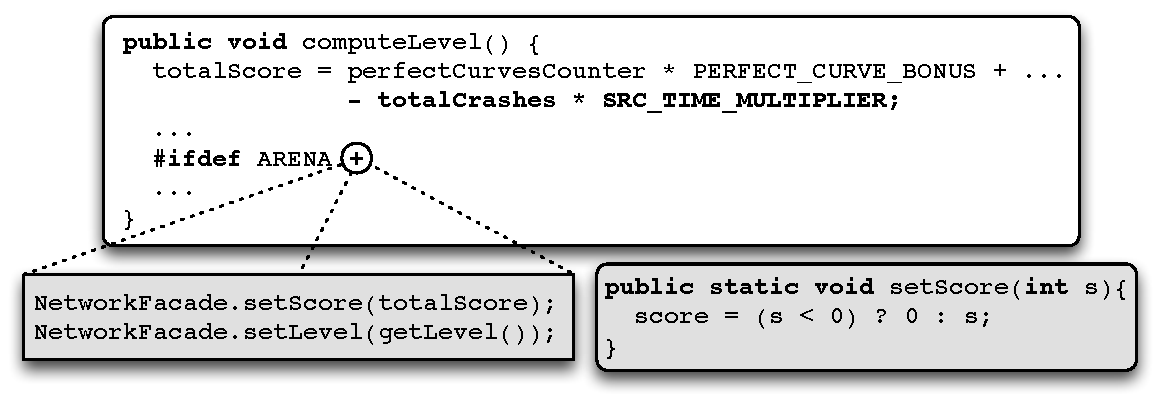
\includegraphics[width=0.5\textwidth]{images/Arena-Example.pdf}
    \caption{Code change only works for some products. \textit{ARENA} feature code in gray.}
    \label{fig:arena-example}
\end{figure}

In this scenario, consider the following planned change.
To add penalties in case the player often crashes the car, let the game score be not only positive, but also negative. To accomplish the task, a developer localizes the \textit{maintenance points}, in this case the \texttt{totalScore} assignment, and changes the computation of scores (see the bold line in Figure~\ref{fig:arena-example}). Products without the \emph{ARENA} feature now enjoy the new functionality, but unfortunately the change is incomplete for products with the \emph{ARENA} feature. In the implementation of feature \emph{ARENA}, method \texttt{setScore} again checks for positive values and unintentionally prevents submitting negative scores to the network server.

The cause of the problem is that the \emph{ARENA} implementation extends the behavior and is therefore affected by the change as well. This was not, however, noticed by the developer, who did not realize that she had to change code associated to other features. In this case, she would have to change part of the \emph{ARENA} code to not check the invariant that all scores are positive. In the actual implementation, feature \emph{ARENA} is partially implemented inside method \texttt{computeLevel} and guarded with \texttt{\#ifdef} directives, so it might not be so difficult to notice the dependency if the method is not so big. 
However, in more complex code or even alternative implementation approaches that separate the feature implementation (see Section~\ref{sec:otherimpl} below) the dependencies across feature boundaries might be harder to track.
%However, we could alternatively implement it in a separate aspect, or keep it hidden through the use of virtual separation. In both cases, for code change tasks that do not obviously relate to feature \emph{ARENA}, the developer could easily miss the dependency.

In this context, searching for cross-feature dependencies might increase developers effort since they have to make sure that the modification does not impact other features. Further, if they miss a dependency, they can easily introduce errors by not properly completing the code change task, for example.

%Building a product with the \textit{ARENA} feature enabled and running it may make the developer incorrectly assume that everything is correct, since the negative total score correctly appears after the race. However, when publishing the score on the network, she notices that the negative score is in fact stored as zero (see the expanded \textit{ARENA} code in gray). Hence, the maintenance was only correctly accomplished for products without \textit{ARENA}.

%The method contains a hidden optional feature, named \textit{ARENA}, responsible for publishing the scores obtained by the player on the network so that players are able to compare their results.

%Also, suppose that the developer is using VSoC, so that there are hidden features throughout the code, including \textit{ARENA}. The developer might well judge that they are not important for this current task. 
%\chk{the following is partially redundant. shorten?}
%So, the developer might be unaware that another feature she is not maintaining uses \texttt{totalScore} and thus also needs to be changed accordingly to correctly accomplish the task. In fact, the impact on other features leads to two kinds of problems. Firstly, due to the incomplete task---the developer should also remove the check from the \texttt{setScore} method---she introduced an \textit{error}. Now, we can only detect this error when we eventually happen to build and execute a product with the problematic feature combination (here, any product with \textit{ARENA}). Secondly, searching for uses of \texttt{totalScore} might increase developers \textit{effort}. Depending on the number of hidden features, the developer needs to consider many locations to make sure the modification did not impact other features. So they might navigate throughout different methods and even different classes, increasing effort.

\subsection{Scenario 2: Fixing an unused variable}
\label{sec:breaks}

Our second scenario is based on a bug report from \textit{glibc}.\footnote{\url{http://www.gnu.org/s/libc/}} This project is structured with several preprocessor macros and conditional-compilation constructs. Developers report that a variable \texttt{status} in the common code base is reported as unused. Investigating the problem, we find that \texttt{status} is declared in all configurations, but only used when features \emph{CHOWN} or \emph{UTIMES} are selected, as shown in Figure~\ref{fig:gfilestatus-example} (left-hand side). When we compile the product line without either feature, the compiler issues an unused-variable warning. 

\begin{figure}[htp]
    \centering 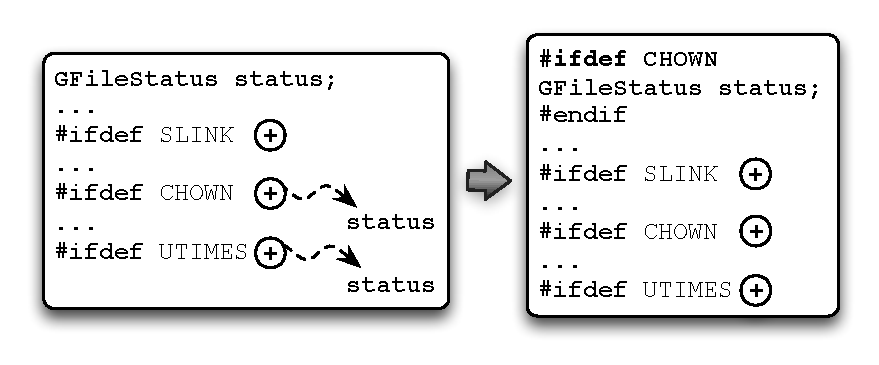
\includegraphics[width=0.4\textwidth]{images/GFileStatus-Example.pdf}
    \caption{Wrong fixing of an unused variable.}
    \label{fig:gfilestatus-example}
\end{figure}

To fix the bug report, a developer would typically look for uses of the variable. If she does not carefully look across feature boundaries, she can easily introduce an error. The problem can even be worse when there are requirements-level dependencies between features, e.g., that \emph{SLINK} cannot be selected without \emph{CHOWN}.

In an unsuccessful attempt to fix the warning, the developer could, for example,  detect only the variable usage in feature \emph{CHOWN}, and then guard the declaration correspondingly as shown in the right-hand side of Figure~\ref{fig:gfilestatus-example}. This would actually lead to a worse problem: an undeclared variable compilation error for configurations with \emph{UTIMES} but without \emph{CHOWN}. The correct fix would require to guard the declaration with \texttt{\#ifdef (CHOWN || UTIMES)}.

%In fact, she solved the unused variable problem but introduced a worse problem: now there is an undeclared variable. Indeed, if we build a product without feature \textit{CHOWN}, we remove the \texttt{status} declaration. Since feature \textit{UTIMES} uses it, the code does not compile for products that contain this feature.

Again, the initial problem and the incorrect fix are caused by the difficulty to follow dependencies across feature boundaries. Again, these are easy to detect in small and simple methods, but might be complicated in larger code bases and other language mechanisms that actually separate the feature code (see Section~\ref{sec:otherimpl} below).

 %This applies not only to preprocessor-based systems and virtual separation environments, but also to systems and product lines structured with other mechanisms. So, in the presence of crosscutting features, identifying feature dependencies may require substantial effort, and missing such dependencies can easily lead to programming errors.

%Because developers can still compile products without the \textit{UTIMES} feature, they did not notice the problem and might generate a release containing it, introducing an \textit{Error} visible only in some out of many configurations, possibly detected only late. Searching for uses of \texttt{status} increases \textit{Effort}.

\subsection{Cross-Feature Dependencies in the Wild}

Initially, the previously shown examples seem pretty specific, requiring preprocessor directives and data-flow dependencies. To quantify their frequency, we have previously conducted a conservative study~\cite{ribeiro-feature-dependencies-gpce11} mechanically mining the code base of $43$ highly configurable software systems with a total of over 30 million lines of code, including \textit{Linux}, \textit{Freebsd}, \textit{postgres}, \textit{sendmail}, \textit{gcc}, and \textit{vim}. All these common open-source systems make heavy use of preprocessor directives for configuration (for features and portability).
Even just looking conservatively at \textit{intraprocedural} data-flow within individual methods, between 1 and 24~percent of all methods in the studied systems contain cross-feature dependencies; however, typically more than half of the methods with \texttt{\#ifdef} directives also contain cross-feature dependencies. These numbers only serve as a lower bound, since \textit{interprocedural} data-flow between methods was not measured but likely causes additional cross-feature dependencies. These results show that the problem, even though quite specific, is so common in practice that building dedicated tool support can be beneficial for a wide range of code change tasks.


%\textbf{TODO: can you add a paragraph or two about the key insights from the GPCE paper?}

\subsection{Beyond preprocessors}
\label{sec:otherimpl}
%Furthermore, code dependencies may cross feature boundaries, so that a variable changed in one feature is read by another feature. A developer must make sure that all of those dependencies are considered as well.

We illustrate the problem for preprocessor-based product lines, but in fact other implementation approaches suffer from limited modularity mechanisms, especially implementation approaches supporting some form of crosscutting. While variability can make cross-feature dependencies harder to detect, it is by no means necessary.

One of the well-known and controversially discussed examples is \emph{aspect-oriented programming} in the style of AspectJ. With AspectJ, code of features (or more generally concerns) is separated into a distinct code unit, the aspect, and reintroduced in a weaving step. The control-flow or data-flow between aspects and base code is not protected by explicit interfaces---a fact for which AspectJ was repeatedly criticized~\cite{storzer-fragile-pointcut-04, S:OOPSLA06}, but which was also discussed as strength enabling flexibility~\cite{filman:oopsla-aop00}.%
\footnote{Several extensions to aspect-oriented languages have been discussed that require declaring explicit interfaces between concerns~\cite{SPAK:TOSEM10,join-point-interfaces-erics-esec-fse11,aldrich-open-modules-ecoop05,GSSSTCR:IEEESoftware06,rajan-ptolemy-ecoop08}; here we take an alternative tool-based approach.} The first example works just as well with an aspect injecting the \emph{ARENA} code instead of an in-place \texttt{\#ifdef} block.

Other structure-driven composition mechanisms, such as \emph{feature-oriented programming}~\cite{batory-refinement-tse04}, \emph{delta-oriented programming}~\cite{delta-ina-splc10}, or even just inheritance with \emph{subclassing}~\cite{fragile-base-class-ecoop98} exhibit similar potential problems.

Finally, also in the context of preprocessor-based implementations, recent advances support some separation of feature code.
To deal with the scattering of feature code in preprocessor-based implementations, researchers have investigated \emph{virtual} forms of separating concerns by helping developers to focus on relevant features~\cite{christian-cide-icse08,ABGM:TSE02,erwig-harmful,HKW:ICSE08}. For example, in CIDE~\cite{christian-cide-icse08}, developers can create \emph{views} on a specific feature selection, hiding irrelevant files and irrelevant code fragments inside files, with standard code-folding techniques at the IDE level. Code fragments are hidden if they do not belong to the selected feature set the developer has selected as relevant for a task. In our examples, we have already shown the collapsed versions of \texttt{\#ifdef} statements with a $\oplus$ marker indicating additional code. Virtual separation in this form has been shown to allow significant understandability and productivity gains~\cite{ABGM:TSE02,erwig-harmful}. However, hiding also has a similar effect as moving code into an aspect: it is no longer visible locally (except for a marker indicating hidden code) and there is no interface describing the hidden code. This way, virtual separation makes the problem of cross-feature dependencies even worse.




%The problem we outline is shared by many implementation approaches for product lines that support some form of crosscutting. For example, if we use aspects (or similar techniques) to implement crosscutting features~\cite{eduardo-empirical-study-icse08}, and configure the product line by selecting which aspects to weave, we need to consider potential dependencies between (optional) aspects and classes. In practice, a more common scenario, and the one we focus here, is to use conditional-compilation (\texttt{\#ifdef} constructs) with a preprocessor, where optional code fragments are merely annotated in a common code base~\cite{liebig-40spls-icse10}. Also in this context, dependencies cross method and feature boundaries and may only occur in specific configurations and are not explicit in interfaces.

%To deal with the scattering of feature code in preprocessor-based implementations, researchers have investigated virtual forms of separating concerns by helping developers to focus on relevant features. For example, in CIDE~\cite{christian-cide-icse08}, developers can create views on a specific feature selection, hiding irrelevant files and irrelevant code fragments inside files, with standard code-folding techniques at the IDE level. Code fragments are hidden if they do not belong to the selected feature set the developer has selected as relevant for a task. While virtual separation with hiding can emulate some form of modularity, it also potentially hides code fragments that might be relevant for code change tasks. Similar to separating features with aspects, a view shows only the code of one feature (or a set of features) while dependencies may point to code in other aspects or hidden code fragments (visible only in other views). Developers are then prone to make errors and need to invest effort to trace dependencies, as we illustrate next with two scenarios.

%!TEX root = ../main.tex

\section{Emergent Interfaces}

\label{sec:emergent}

%%%%%%%%%%%%%%%%%%%%%%%%%%%%%%%%%%%%%%%%%%%%%%%%%%%%%%%%%%%%%%%%%%%%%%%%%

The problems discussed so far occur when features \textit{share} elements such as variables and methods, raising cross-feature dependencies. For instance, the common base code might declare a variable subsequently used by an optional feature (see \texttt{totalScore} and \texttt{status} in Figures~\ref{fig:arena-example} and~\ref{fig:gfilestatus-example}, respectively).

In this context, there are several paths to attack the problem with unclear cross-feature dependencies outlined in the previous section. The typical language-designer approach is to introduce additional modularity concepts into the programming language and make control-flow and data-flow explicit in interfaces, such as~\cite{shriram}. With \emph{emergent interfaces}, we pursue an alternative tool-based direction, which also works with existing languages and existing implementations and infers interfaces on demand.

%usar data flow na definicao. Em seguida, falar algo como: ``although we focus on data flow, we could use in control flow etc." Falar tambem que o Emergo so pegs dataflow.

To better explain what is an emergent interface, we first introduce maintenance points. \textit{Maintenance points are the code lines that the developer wants to change, for which she is interested in the cross-feature dependencies.} Also, we name \textit{impacted points the code lines we potentially impact if we change the maintenance points}. As any other code line, all these lines might be associated with feature expressions by using \texttt{\#ifdef} statements. Notice that one maintenance point---one code line---may impact many other code lines.

To define an emergent interface, let $MP$ be the set of maintenance points and $IP$ be the set of potentially impacted points. Also, let $FE(line)$ be a function that returns the feature expression associated with a given code line. This way, \textit{an emergent interface is a list of contracts in terms of ``$IP_i$ requires $MP_j$" emerging only if $FE(MP_j) \not\equiv FE(IP_i)$ and $FE(MP_j) \wedge FE(IP_i)$ is a valid feature expression}. Notice that for each contract of the list we have two elements: the maintenance point (the one that \textit{provides} data); and the impacted point (the one that \textit{requires} data). In other words, an emergent interface contains a list of contracts stating the code lines data dependent on the maintenance points. However, to emerge, each contract of the list must satisfy two constraints: the maintenance point and impacted point must have not equivalent feature expressions; and the conjunction of these expressions must be valid. The not equivalent constraint is necessary to compute cross-feature dependencies and the conjunction constraint prevents developers from assuming invalid dependencies.

Now, when developers are interested in dependencies from specific maintenance points, they can ask the tool that implements the technique to compute interfaces, pointing out feature dependencies. The interfaces emerge on demand, giving support for developers to maintain one feature without breaking others, since now they are aware of cross-feature dependencies. That is, the interfaces are inferred and shown in the IDE environment, instead of being written manually by developers.

To better illustrate how emergent interfaces work, we now refer to Figure~\ref{fig:eis}, which illustrates two maintenance tasks. When considering task~1, suppose there is something wrong with the initialization of variables \texttt{x}, \texttt{y}, and \texttt{k}. So, we should change them. Regarding task~2, we should change the \texttt{return} expressions of function \texttt{h}. For task~1, we select the following maintenance points (see the non-contiguous lines in dashed rectangles): lines $12$, $13$, $14$, and $27$ of \texttt{File F1}; afterwards, for task~2, we select lines $83$ and $85$ of \texttt{File F2}. 

%Figure~\ref{fig:eis} also makes explicit some feature constraints: features \texttt{A} and \texttt{B} are mutually exclusive; and feature \texttt{F} requires \texttt{!C}. Notice that this information might not be explicit in source code.

The emergent interfaces for tasks~1 and~2 contain six contracts and one contract, respectively. Each interface details, for each maintenance point, the potentially impacted statement, its line, its file, and the feature configuration in which the maintenance point impacts such a statement. We assume that the dots ``$\dots$" in Figure~\ref{fig:eis} do not contain any assignment to the variables we are interested during our maintenance tasks.

According to the emergent interface 1, if we change the statement \texttt{int x = 0} we impact the statements in lines $53$ and $87$, since they use the value of \texttt{x} and there is no path from the maintenance point to these lines where we assign a new value to \texttt{x}. Because we impact the statement \texttt{z = x + 9}, we transitively impact line $88$---\texttt{print(z)} statement---, since our maintenance in variable \texttt{x} contribute to define the value of \texttt{z} as well. This happens when we enable features \texttt{B}, \texttt{C}, and \texttt{D} (see column ``Feature Config."). When considering \texttt{y = g()} we impact line $87$ in products with \texttt{!A \&\& C \&\& D}. Due to the new assignment to \texttt{y} in feature \texttt{A}, this situation only occurs in case feature \texttt{A} is not enabled. Finally, if we change the assignment to variable \texttt{k} in line $14$ we impact lines $27$ in \texttt{File F1} and $33$ in \texttt{File F2}. To impact line $33$, the product must have feature \texttt{B} enabled and feature \texttt{E} not enabled. Notice that the maintenance point \texttt{k++} does not impact any line, including \texttt{i(k)}. According to the feature constraints at the bottom of Figure~\ref{fig:eis}, features \texttt{A} and \texttt{B} are mutually exclusive, so they do not impact each other. Therefore, we do not emerge any contract for this case---$FE($\texttt{i(k)}$) \wedge FE($\texttt{k++}$) = A \wedge B$ is not valid---preventing developers from assuming a non-existing dependency. Notice that constraints like this one might not be explicit in source code or even are unknown by developers.

According to the emergent interface 2, we impact only one point, i.e., line $87$ in \texttt{File F1}. The statement \texttt{return m + n} impacts the call to function \texttt{h} in products with \texttt{!F \&\& C \&\& D}. The statement \texttt{return m} does not impact such a call because if we enable feature \texttt{F}, we must disable feature \texttt{C} (see the constraint in Figure~\ref{fig:eis}).

Now, because developers are aware of cross-feature dependencies pointed by the emergent interface, they have better chances of not introducing errors to the code lines dependent on the maintenance points. In addition, developers do not need to reason about feature constraints hardly ever explicit in code; emergent interfaces already does it. Emergent interfaces also bring benefits to virtual separation and even for testing activities. We can improve comprehensibility (we hide the features not dependent of our task and focus on the ones we really care) and reduce effort by testing only the feature configurations pointed by our interfaces.

The tool we present next compute interfaces for a given set of maintenance points, helping developers to make code changes once they identify these points. Emergent interfaces do not contribute to finding the maintenance points in the first place, through.

%So, our interfaces play an important role on avoiding conflicts: by looking and analyzing the emergent interface, developers may have better chances of not introducing errors to the code lines dependent on the maintenance points. Thus, we provide treaties among features to resolve conflicts caused by cross-feature dependencies.

%To compute emergent interfaces, we use a feature-based slicing, which means we take feature constraints into account. We show the emergent interfaces for each task at the right-hand side of Figure~\ref{fig:eis}.

\begin{figure*}[ht]
\centering
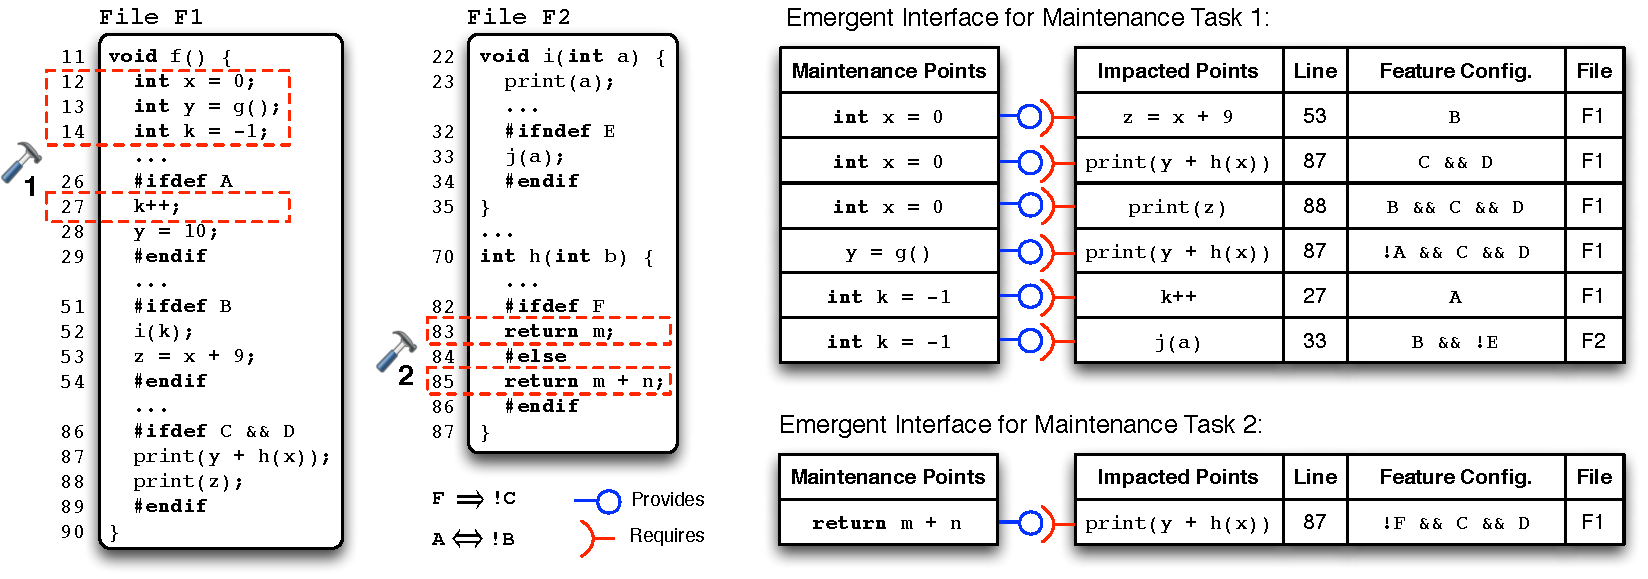
\includegraphics[width=0.92\textwidth]{images/EIs.pdf}
\caption{Examples of maintenance points and their respective emergent interfaces.}
\label{fig:eis}
\end{figure*}

%%%%%%%%%%%%%%%%%%%%%%%%%%%%%%%%%%%%%%%%%%%%%%%%%%%%%%%%%%%%%%%%%%%%%%%%%

%Now, we return to our scenarios from the previous section, using preprocessor-based implementations and views of virtual separation. 

%The problems discussed so far occur essentially because features \textit{share} values and behavior without clear interfaces. Whenever we have such sharing in the control flow or data flow, we say that there is a code level \textit{feature dependency} between the involved features~\cite{ribeiro-feature-dependencies-gpce11}. For instance, a mandatory feature might declare a variable subsequently used by optional features (see \texttt{totalScore} and \texttt{status} in Figures~\ref{fig:arena-example} and~\ref{fig:gfilestatus-example}, respectively).

%There are several paths to attack the problem with unclear cross-feature dependencies outlined in the previous section. The typical language-designer approach is to introduce additional modularity concepts into the programming language and make control-flow and data-flow explicit in interfaces, such as~\cite{shriram}. With \emph{emergent interfaces}, we pursue an alternative tool-based direction, which also works with existing languages and existing implementations and infers interfaces on demand.

%Emergent interfaces establish, on demand and according to a given code change task, interfaces to feature code. We use the following notion of interface: ``an interface is a way to resolve potential conflicts between the interacting parts of a design"~\cite{clark-design-rules-00}. Thus, we provide treaties among features to resolve conflicts caused by cross-feature dependencies. For example, an interface may state that a feature \textit{reads} a variable \textit{modified} by another.

%When developers are interested in dependencies from a specific code block, they can ask the tool that implements the technique to compute interfaces, pointing out feature dependencies. The interfaces emerge on demand, giving support for developers to maintain one feature without breaking others. That is, the interfaces are inferred and shown in the IDE environment, instead of being written manually by developers.

%To illustrate how emergent interfaces work, we return to our scenarios from the previous section, using preprocessor-based implementations and views of virtual separation. Consider \textit{Scenario 1}, where the developer is supposed to change how the total score is computed. The first step when using our approach consists of selecting the \emph{maintenance points}. A maintenance point is the point that the developer wants to change, for which she is interested in the interfaces to other features. In our case, the developer  manually selects the \texttt{totalScore} assignment as maintenance point (see the dashed rectangle in Figure~\ref{fig:arena-ei}) and then our tool analyzes the code to capture dependencies between the feature she is maintaining and the others. Finally, the interface emerges as shown in Figure~\ref{fig:arena-ei} (right-hand side).

%\begin{figure}[htp]
%\centering
%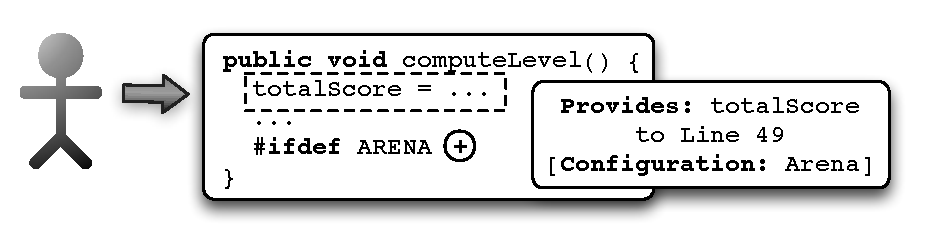
\includegraphics[width=0.45\textwidth]{images/Arena-EI.pdf}
%\caption{Emergent interface for Scenario 1.}
%\label{fig:arena-ei}
%\end{figure}

%The emerged interface states that the code change task may impact the behavior of products containing the \textit{ARENA} feature. So, the common code base provides \texttt{totalScore} current's value whereas \textit{ARENA} requires it. The developer is now aware of the dependency. When investigating it, she is likely to discover that she also needs to modify \textit{ARENA} code to avoid introducing an error.

%The tool we present next always compute interfaces for a given set of maintenance points, helping developers to make code changes once they identify these points. Emergent interfaces do not contribute to finding the maintenance points in the first place, through.

%Notice we do \textit{not} provide any support to find the maintenance points. This task is up to the developer according to her knowledge about the source code. After finding these points, she takes them as input to our approach. Then, we provide information about the potential features she might impact.

%This way, EIs focus on the features we indeed might impact, avoiding developers from the task of analyzing unnecessary features, being important to decrease \textit{Effort}. For instance, consider \textit{Scenario 2} (Section~\ref{sec:breaks}) in which we use the \texttt{status} variable in two optional features. Here, our interface ignores the \textit{SLINK} feature, since it does not use the \texttt{status} variable. Now, the navigation throughout the code is easier.

\subsection{Implementation: Emergo}

We implemented the concept of emergent interfaces in an Eclipse-based tool named Emergo. Emergo computes emergent interfaces based on feature dependencies between methods or within a single method, by using \textit{interprocedural} or \textit{intraprocedural} feature-sensitive data-flow analysis~\cite{brabrand-dfa4spl-aosd12, bodden-ifds4spl-pldi13}. This means we can take only valid feature combinations into account, preventing developers from reasoning about feature constraints and even from assuming invalid dependencies in case of mutually exclusive features (which may cause potential errors). Again, developers might assume that changing the \texttt{k++} assignment in feature \textit{A}---in Figure~\ref{fig:eis}---may lead to problems in feature \textit{B} (see the \texttt{i(k)} statement). Since the involved features are mutually exclusive, Emergo would not emerge any interface, which means that code change tasks in the former feature do not impact the latter, and vice-versa.

%\begin{figure}[htp]
%\centering
%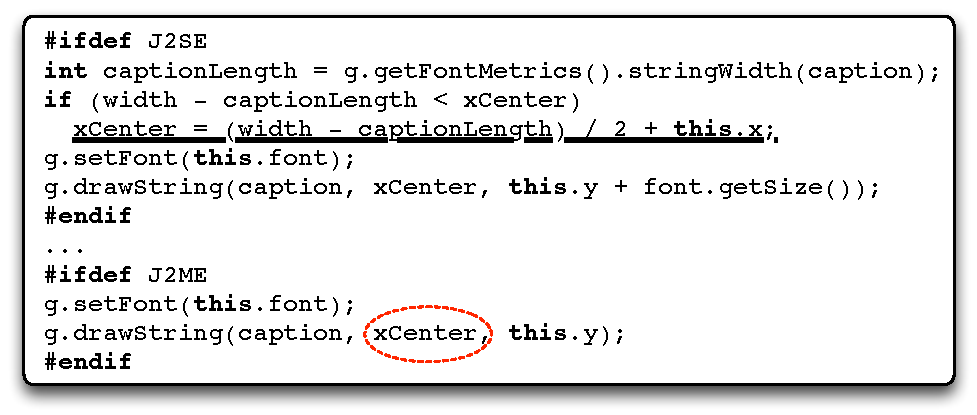
\includegraphics[width=0.5\textwidth]{images/Alternative.pdf}
%\caption{No dependency: mutually exclusive features.}
%\label{fig:emergo-alternative}
%\end{figure}

To illustrate Emergo in action, we return to our scenarios from the previous section. Consider \textit{Scenario 1}, where the developer is supposed to change how the total score is computed. The first step when using our approach consists of selecting the \emph{maintenance points}. In our case, the developer manually selects the \texttt{totalScore} assignment as maintenance point. Then, she would rely on Emergo to analyze the code to capture dependencies between the feature she is maintaining and the others. Finally, the interface emerges stating that the code change task may impact the behavior of products containing the \textit{ARENA} feature. So, the common code base provides \texttt{totalScore} current's value whereas \textit{ARENA} requires it. The developer is now aware of the dependency. When investigating it, she is likely to discover that she also needs to modify \textit{ARENA} code to avoid introducing an error.

Figure~\ref{fig:emergo} illustrates a screen shot of Emergo. After the developer found and selected the maintenance point in Line~1277 (the \texttt{totalScore} assignment), Emergo shows emergent interfaces using a table view and a graph view. To better understand the results pointed by Emergo, we now focus on the table. The ``Description" column illustrates the maintenance points. Since there is no \texttt{\#ifdef} statement encompassing the maintenance point, we associate it with the \textit{mandatory} feature. We show the potentially impacted configuration in the ``Feature" column, here with the \textit{ARENA} feature. The table view also shows the exact (impacted) lines of code that contain uses of \texttt{totalScore} as well as their respective files (see the ``Resource" column). In summary, we read the first line of the table as follows: if she changes the \texttt{totalScore} assignment belonging to the mandatory feature, she can potentially impact products with the \textit{ARENA} feature in line 177 of the \texttt{NetworkFacade} class.

Initially, Emergo shows all dependencies in both views. This way, depending on the project, it points lots of dependencies, which might be difficult to read and understand them. Thus, to focus on a particular one, she can click on the corresponding table line and Emergo automatically removes unrelated dependencies of the graph. This means we only show the path associated with the dependency of that table line. According to Figure~\ref{fig:emergo}, she selected the first line of the table. So, the graph now has only the path from the maintenance point to line 177 of the \texttt{NetworkFacade} class. 

Also, developers can reach the impacted feature code in the IDE editor by clicking either on table lines or on the graph nodes. For example, if she clicks on the node ``\texttt{score = (s < 0) ? 0 : s;}" of the graph, she reaches the code that checks the invariant that all scores are positive. Now, she is aware of the dependency. So, to accomplish the task of allowing negative scores she knows she also needs to remove the check.

\begin{figure*}[ht]
\centering
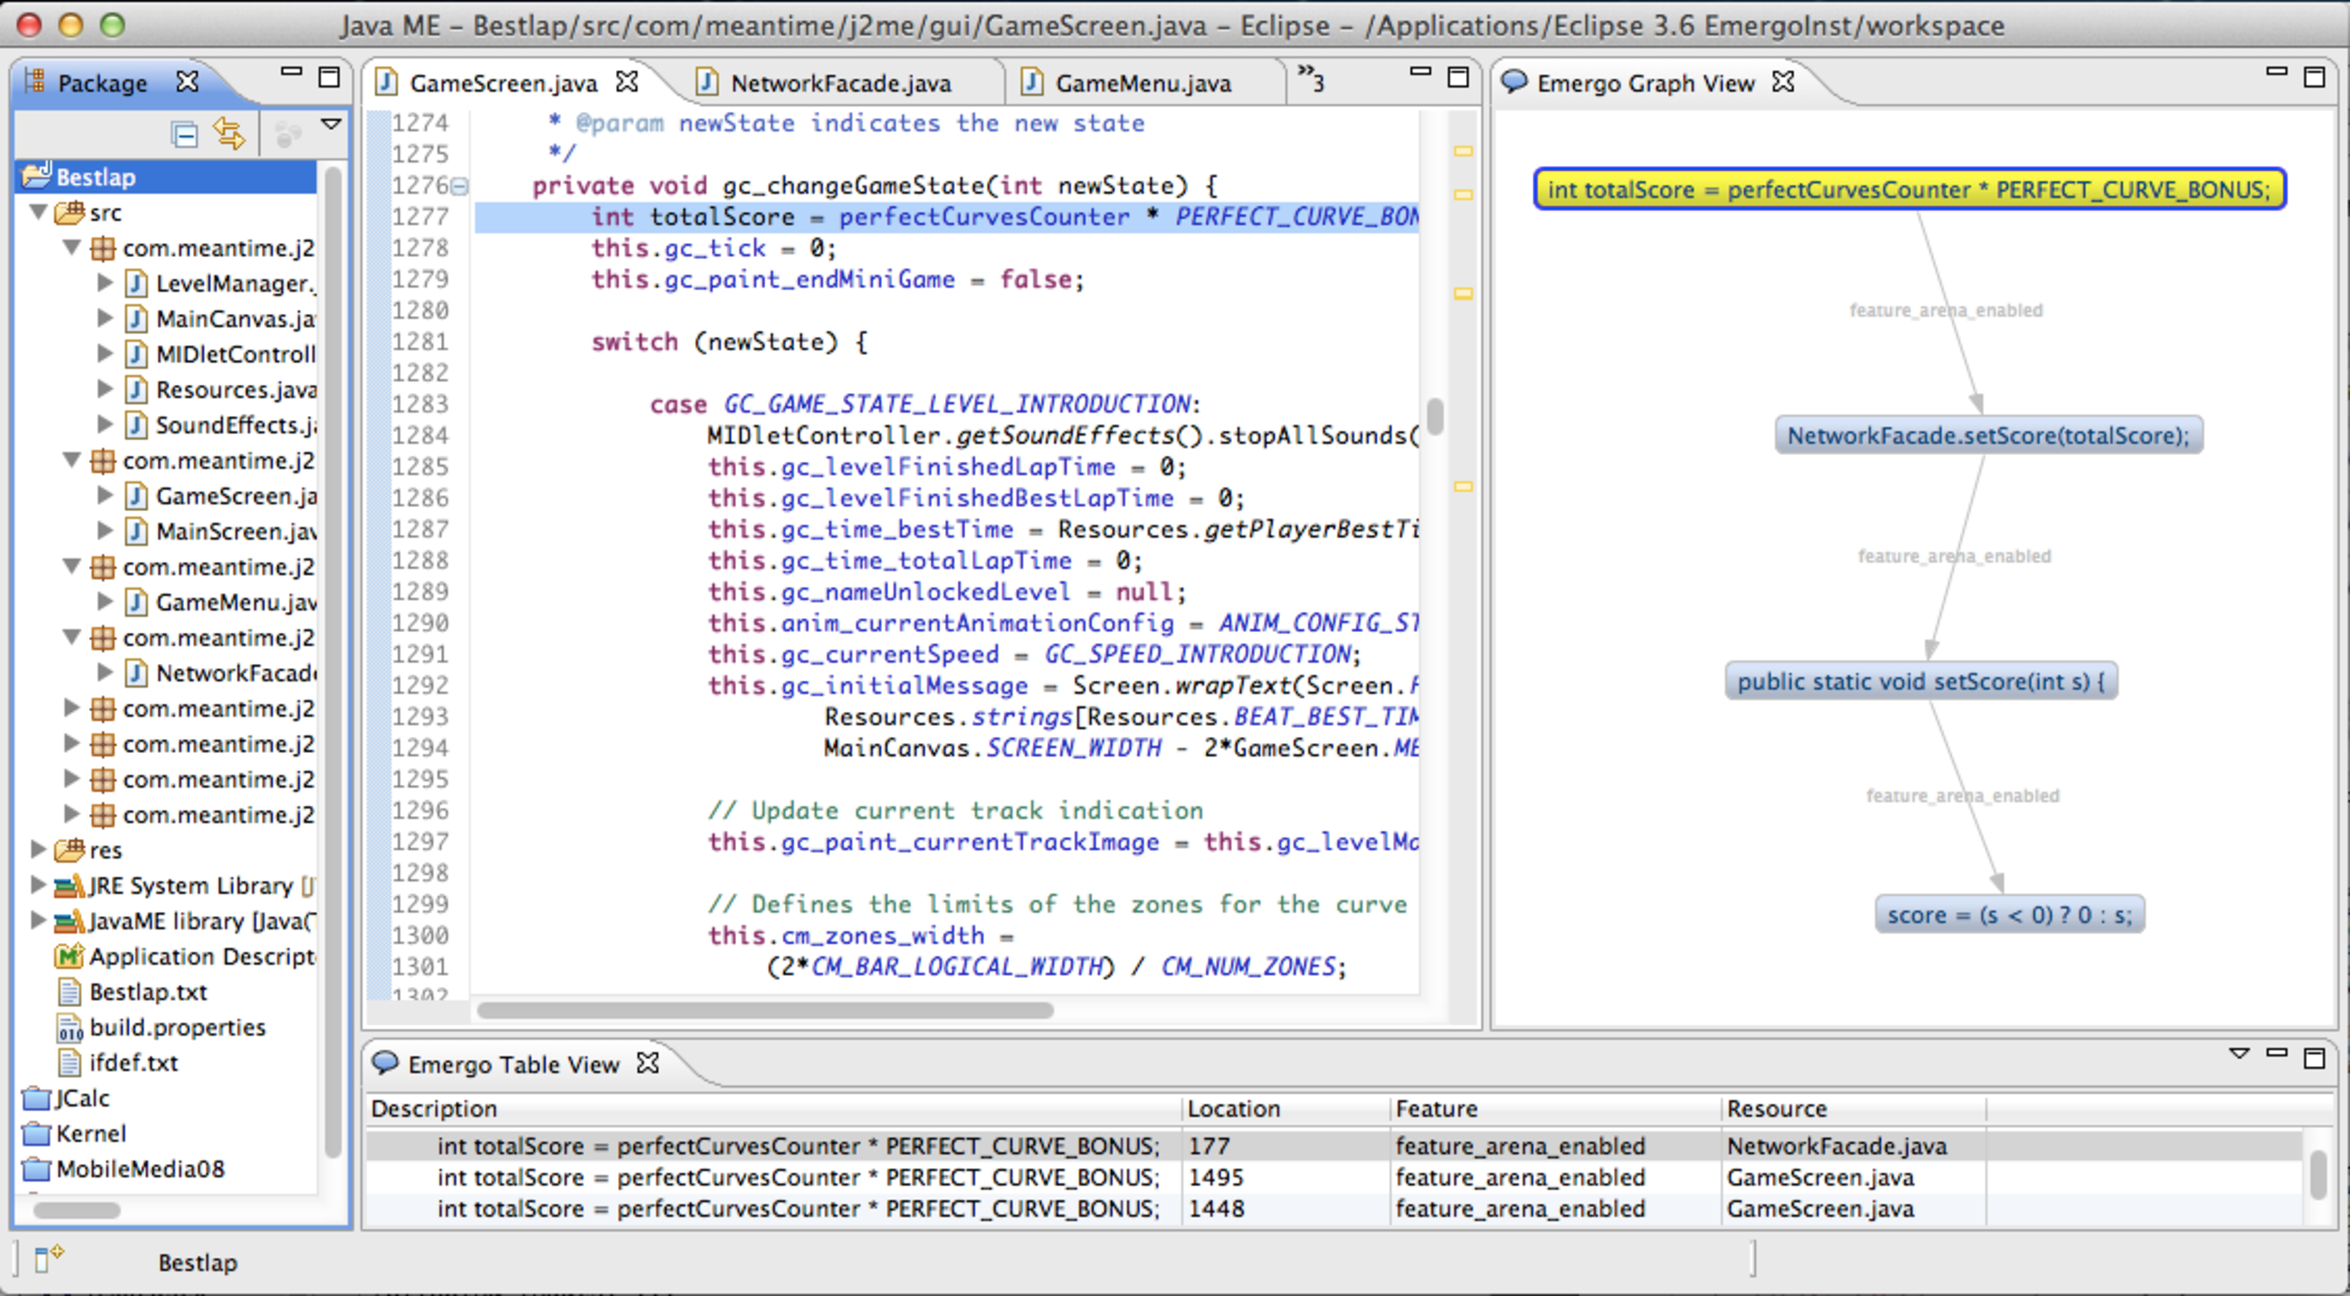
\includegraphics[width=.9\textwidth]{images/Emergo.pdf}
\caption{Emergent interface for Scenario 1 using Emergo.}
\label{fig:emergo}
\end{figure*}

Emergo can also help on preventing developers from analyzing unnecessary features and their associated code, which is important to decrease code change effort. In particular, we believe that Emergo can help on making the idea of virtual separation of concerns realistic. Thus, we can hide features and rely on Emergo to only open the ones we really need to. For instance, consider \textit{Scenario 2} (Section~\ref{sec:breaks}). Emergo would focus on \textit{CHOWN} and \textit{UTIMES}. So, we could keep \textit{SLINK} hidden, since it is not related to the current task.

Currently, our implementation has some limitations. To compute dependencies, we rely only on data-flow information, so we only compute data dependencies. Also, developers can only select maintenance points that range from simple variable assignments to code blocks that do not span to another method.

%containing assignments, method calls, and variable (local or class attributes) and method declarations. To compute interfaces for declarations, we also rely on AST-based analyses.

\subsection{Underlying Analysis}

The current implementation of Emergo computes interfaces based on data using \textit{interprocedural} and \textit{intraprocedural} feature-sensitive \textit{reaching-definition analysis}. So, from the maintenance points, we consider the reached program statements and their associated feature expressions to form our emergent interfaces. The feature-sensitive approach is capable of analyzing all configurations of a product line without having to generate all of them explicitly. This increases performance~\cite{brabrand-dfa4spl-aosd12, bodden-ifds4spl-pldi13}, which is important for interactive tools like ours that need to provide quick responses to developers requests. To perform the feature-sensitive analysis, we annotate the control-flow graph with feature information, lift the lattice to contain a mapping of sets of configurations to lattice values, and lift the transfer functions to figure out whether or not apply the ordinary function. The lifted function lazily splits the sets of configurations in two disjoint parts, depending on the feature expression annotated with the statement being analyzed: a set for which the function should be applied; and a set for which it should not~\cite{brabrand-dfa4spl-taosd12}.

%The current implementation of Emergo computes interfaces based on data using \textit{interprocedural} and \textit{intraprocedural} feature-sensitive reaching definition analysis. We also rely on AST-based analyses.

%\textbf{TODO explain in one or two paragraphs what kind of analysis is performed. move technical content from the previous section here.}

%\reviewer{Rev2: With regards to the technique of expressing and computing emergent interfaces, it is unclear what the input to the technique is. Is it a specific variable? A variable at a particular point in the code? An entire code block? A code block that spans more than one method? I would like to see much more clarity on the inputs to the mehod than provided by:}

%\reviewer{Figure 4 also made me question what the inputs and outputs are. How is the impacted feature shown? What is the feature in this example?}

%\idea{Maybe we should consider a complete screen shot of Emergo, instead of only considering the table view. We can do it since now we have some extra pages: 10 (icse) x 14 (oopsla).}

%\begin{figure}[htp]
%\centering
%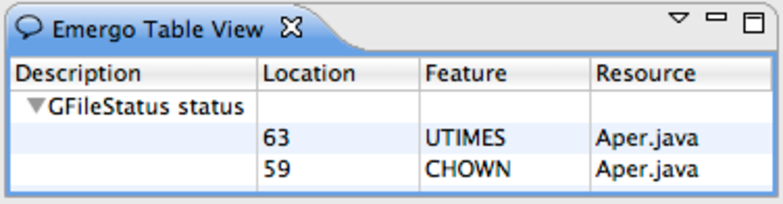
\includegraphics[width=0.45\textwidth]{images/Emergo-Table-View.pdf}
%\caption{Emergo view illustrating the impacted features. Lines 63 and 59 contain uses of \texttt{status}.}
%\label{fig:emergo-table-view}
%\end{figure}

%\reviewer{Rev1: That said, section III felt too short, especially if you have extended the tool. Some words on that and how it works would help.}

%\chk{from the description it is not clear how emergent interfaces are computed. you just say dataflow analysis, but that's probably littel help. you might want to describe at least in a few words when Emergo reports something, and how the analysis figures that out. possibly you might need to show a dataflow graph for one of the examples.}

%!TEX root = ../main.tex

\section{Experimental design}

\label{sec:experimental-design}

In the previous section we suggest that emergent interfaces can make feature code change tasks (such as \textit{Scenario 1} and \textit{Scenario 2}) faster and less error prone. To evaluate these hypotheses and to get a better understanding of the benefits and drawbacks of emergent interfaces, we conducted and replicated a controlled experiment. We specifically investigate and compare code change effort and introduced errors when maintaining preprocessor-based product lines with and without our interfaces in a setting that supports virtual separation, allowing developers to hide feature code fragments.

\subsection{Goal, Questions, and Metrics}

Our evaluation aims to compare maintenance of preprocessor-based product lines with and without emergent interfaces (these are our treatments). Specifically, we are interested in the interaction with the feature hiding facilities of virtual separation of concerns, which we enable in both cases to aid comprehensibility. We evaluate emergent interfaces from the developer's point of view and observe effort and number of errors they commit. We investigate the following questions:

\begin{itemize}

	\item Question 1: \textit{Do emergent interfaces reduce effort during code change tasks involving feature code dependencies in preprocessor-based systems?}
	
	\item Question 2: \textit{Do emergent interfaces reduce the number of errors during code change tasks involving feature code dependencies in preprocessor-based systems?}

\end{itemize}

To answer Question~1 (effort), we measure the time required to find cross-feature dependencies and to change the impacted features to accomplish a code change task. Figure~\ref{fig:workflow-time} illustrates our setup with and without emergent interfaces.
Note that our setup does not measure the time needed to find the maintenance point (we actually provide the maintenance point with our task description as we describe below). While finding the maintenance point may dominate the entire tasks in a real-world setting, emergent interfaces do not contribute to that part. Hence, we measure only the part of the maintenance task after the maintenance point was identified. This focus of our measurement eliminates noise that would not contribute to our analysis. 

%We do not count the time to find the maintenance points. One might argue that the time to locate them is not negligible. However, given that our idea supports developers to better understand the impact of their changes, counting the time to locate such points would introduce bias to our evaluation. We claim we are still evaluating an important step of a maintenance task: the code change part. In other words, the implementation part. 

%In our experiments we measure only the implementation part of a maintenance task: the code change task (with or without emergent interfaces). This means we pre-select the maintenance points for the participants. One might argue that the time to locate the maintenance point is not negligible. However, measuring the time to find it would introduce bias. 

\begin{figure}[tp]
    \centering 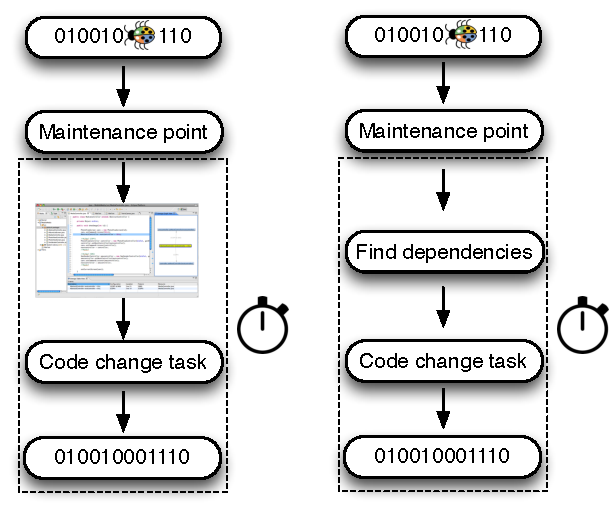
\includegraphics[width=0.35\textwidth]{images/Workflow-Time.pdf}
    \caption{Dashed rectangles represent the time we count (with and without emergent interfaces).}
    \label{fig:workflow-time}
\end{figure}

To answer Question~2 (correctness), we measure how many incorrect solutions the developer committed during a code change task (metric number of errors, or short NE). We consider error as a human action that introduces one or more defects to the code. 
As described below, for some tasks, we provide automated feedback to our participants, so the participant can retry after an incorrect attempt. Other tasks are evaluated manually after the experiment, so participants have only one attempt.

\subsection{Participants}

We performed the experiment in three rounds. In a first pilot study, we tested the experimental design with a small group of six graduate students at the University of Marburg, Germany. Next, we performed the actual experiment with 10 graduate students at Federal University of Pernambuco, Brazil (\textit{Round~1}). Finally, we replicated the experiment with 14 undergraduate students at Federal University of Alagoas, Brazil (\textit{Round~2}). In both rounds, around half of the participants had professional experience---varying from few months to many years of experience---and were actually part-time students. The 10 graduate students are attendants of a course on experimental software engineering lead by an independent lecturer. The 14 are UROP (Undergraduate Research Opportunity Program) students and volunteered to participate. All took part voluntarily and were informed they could stop participating at any time, but nobody did.

\subsection{Material and Code Change Tasks}

We use two preprocessor-based product lines as experimental material: \textit{Best Lap} and \textit{MobileMedia}. The former is a highly variant commercial product line that has approximately 15 KLOC. The latter is a product line for applications with about 3 KLOC that manipulate photo, music, and video on mobile devices~\cite{eduardo-empirical-study-icse08}. It contains feature restrictions and has been used in previous research studies~\cite{eduardo-empirical-study-icse08, rashid-ao-mm}.

We ask participants to perform a number of code change tasks in each of the product lines. Therefore, we provide the product line's source code and corresponding tasks that the participants should perform by modifying the source code. We selected tasks that are particularly affected by cross-feature dependencies, where we expect that our tool can contribute to a better understanding. Note that emergent interfaces target a specific class of problems; for other maintenance tasks we would not expect any benefit. We believe that our task selection can represent typical cross-feature problems as outlined in Section~\ref{sec:motivating}.

To cover different use cases, we prepare two kinds of tasks. In line with our motivating scenarios in Section~\ref{sec:motivating}, we distinguish between tasks where participants should implement a new requirement (requiring \textit{interprocedural} analysis of the existing source code) and tasks where participants should fix an unused variable (requiring only \textit{intraprocedural} analysis). We provide a task of each kind for each product line, for a total of four distinct tasks, as discussed in the following. All task descriptions are available online, see Appendix~A.

\paragraph{Task 1 - New requirement for Best Lap}

The new requirement for \textit{Best Lap} is similar to our motivating \textit{Scenario~1}, but differently from it, there are two methods of feature \textit{ARENA} that contain conditional statements forbidding negative scores. So, to accomplish the task, besides changing the \texttt{totalScore} assignment, participants should remove or rewrite these conditional statements (see one of them in method \texttt{setScore} of Figure~\ref{fig:arena-example}). To reach them, participants need to consider \textit{interprocedural} dependencies. That is, there are dependencies from the maintenance point to two conditional statements, each one in a different method.

In case Emergo is available, the participant should use it to identify the cross-feature dependencies between the variable \texttt{totalScore} and the rest of the code. Otherwise, the participant is free to use standard tools such as find/replace and  highlighting. This also holds for the subsequent tasks.

\paragraph{Task 2 - New requirement for MobileMedia}

The task for \textit{MobileMedia} is conceptually similar in the sense that participants should change a variable assignment, follow feature dependencies, and update conditional statements (here, only one \texttt{if} statement). However, differently from Task 1, where the method call depth to reach the two conditional statements is 1, here the call depth is 2. That is, from the maintenance point, we need to follow two method calls to reach the \texttt{if} statement.

%in that participants should change a variable and all dependencies (with or without Emergo). In \textit{MobileMedia}, participants should replace the actual address of a web server that delivered images with the address of a server that delivered different kinds of documents (including PDF files). The variable they should change is \texttt{server}. However, the change has a rippling effect that touches also upon the implementation of feature \emph{ZOOM}. Previously zoom functionality was only available for vector graphics, but should now also be supported for PDF files. Thus, to accomplish the task, participants should also update the \texttt{if} statement to take this new vector format into consideration. 

%\begin{table}[htb]
%\centering
%\footnotesize
%\begin{tabular}{|c|c|c|c|c|}
%\hline
% & \textit{\textit{Best Lap}} & \textit{\textit{MobileMedia}} \\
%\hline
%Fragments to change & 2 & 1\\
%\hline
%Method call depth & 1 & 2\\
%\hline
%Impacted feature & \textit{arena} & \textit{zoom}\\
%\hline
%Method LOC & 165 & 85\\
%\hline
%Number of Fragments & 4 & 5\\
%\hline
%Number of Features & 2 & 3\\
%\hline
%\end{tabular}
%\normalsize
%\caption{Summary of the \textit{New requirement} tasks characteristics.}
%\label{tab:m1-characteristics}
%\end{table}

\paragraph{Task 3 - Unused variable in Best Lap}

In \textit{Best Lap}, we asked participants to fix the unused-variable warnings for two variables: \texttt{tires} and \texttt{xP}. Such warnings are commonly found in many bug reports of preprocessor-based systems.\footnote{See \url{https://bugzilla.gnome.org/show_bug.cgi?id=461011}, \url{https://bugzilla.gnome.org/show_bug.cgi?id=167715}, \url{https://bugzilla.gnome.org/show_bug.cgi?id=401580}, \url{https://bugzilla.kernel.org/show_bug.cgi?id=1664}} We introduced the bugs ourself by removing correct \texttt{\#ifdef} directives around the variable declarations. We can solve all unused-variable tasks by following \textit{intraprocedural} dependencies only, but they typically require investigating code of different features. To accomplish the tasks, we ask participants to put a correct \texttt{\#ifdef} around the variable declarations. The variables \texttt{tires} and \texttt{xP} are inside methods with 147 and 216 source lines of code, respectively. 

\paragraph{Task 4 - Unused variable in MobileMedia}

Again the \textit{MobileMedia} task is conceptually similar to the \textit{Best Lap} task. Participants should fix the unused-variable warning of \texttt{numberOfViews} and \texttt{albumMusic}. The two variables are placed in shorter methods when compared to Task 3: they have 49 and 71 lines of code. The longest method here has less than half of the lines of the shortest one  in Task 3. 

Emergo computes dependencies for these tasks using \textit{def-use} chains based on the reaching definitions analysis. Thus, it points \textit{intraprocedural} and \textit{interprocedural} dependencies when maintaining a definition used by another feature.

Overall, the tasks for both product lines have similarities, but they are not equivalent. Actually, these differences---methods size, method call depths to reach the impacted feature, and number of conditionals to change---between task for both product lines help us to better analyze the effects of our two treatments and is properly controlled by our experiment design, as we shall see in Section~\ref{sec:design}.

%\reviewer{On what basis do you believe they are comparable? Were they of comparable difficulty to the participants in the study?}

%\reviewer{(I have added a paragraph on this above and we should discuss this in 5.3, otherwise we are fine) Second, I do not mind that the tasks used were simple in nature, however, I do think the type of tasks (the types of changes that were required) were extremely skewed to show the benefits of the tool. It is not realistic to evaluate a tool that highlights hidden dependencies using a scenario where the variable that has the hidden dependencies has been pre-selected for the developers. I would contend that these tasks are by no means representative of real tasks, even small ones.}

Finally, we designed warmup tasks on a toy product line so that participants could learn how to generate emergent interfaces using Emergo at the start of the experiment. We perform warmup tasks together in a class context and are not evaluated.

\subsection{Hypotheses}

Based on our goals and tasks, we evaluate the following hypotheses:

%When using emergent interfaces, developers are aware of features dependencies. This might lead them to find dependencies quickly and, consequently, they can accomplish the task faster.
\begin{itemize}

	\item \textit{H1 - Effort:} With emergent interfaces, developers spend less time to complete the code change tasks involving feature dependencies in both product lines.

%Since developers are aware of dependencies, the probability of changing the impacted features increases, leading them to not submit incomplete tasks.
	\item \textit{H2 - Error introduction:}  With emergent interfaces, developers commit less errors in both product lines when performing the code change tasks involving feature dependencies.

\end{itemize}

\subsection{Design}

\label{sec:design}

To evaluate our research questions, we distinguish between participants using our treatments (independent variable with two levels: with and without emergent interfaces). Additionally, we distinguish between the tasks of both product lines, as we cannot assume equivalence (independent variable with two levels: \textit{Best Lap} and \textit{MobileMedia} tasks). We measure time and the number of errors (dependent variables) for new-requirement tasks and unused-variable tasks.

Since we have two independent variables with two levels each, we use a standard \emph{Latin Square design}~\cite{box-statistics-for-experimenters}. We randomly distribute participants in rows and product lines tasks in columns. The treatments come inside each cell. Each treatment appears only once in every row and every column (see Figure~\ref{fig:latin-squares}). As a result, each participant performs both kinds of tasks on each product line and also uses and not uses emergent interfaces at some part of the experiment, but no participant will perform the same task twice, which avoids corresponding carry-over effects, such as learning (if we let one to use both treatments in the same task, we would favor the second treatment, since she already knows how to accomplish the task). The design does not favor any treatment and blocks two factors: participant and code change tasks.

\begin{figure}[tp]
    \centering 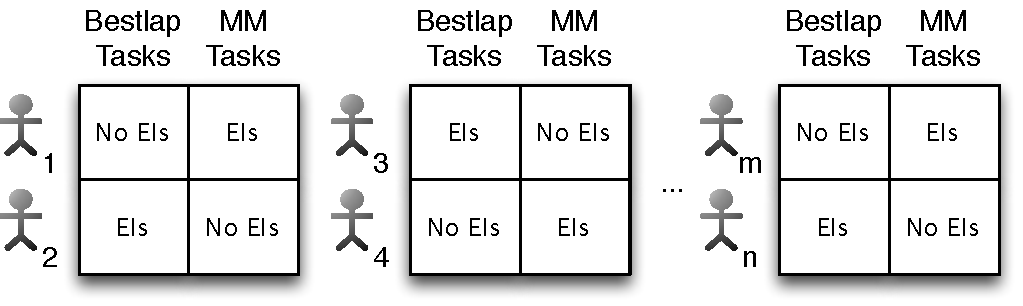
\includegraphics[width=0.48\textwidth]{images/Latin-squares.pdf}
    \caption{Layout of our experiment design: Latin squares.}
    \label{fig:latin-squares}
\end{figure}

As analysis procedure for this design, we perform an analysis of variance (ANOVA). The test compares the effect of the treatments on the dependent variables. To give relevance to the ANOVA~\cite{box-statistics-for-experimenters}, we use the Bartlett, Box Cox, and Tukey tests to verify variance homogeneity, normal distribution, and model additivity, respectively. We follow the convention of considering a factor as being significant to the response variable when \textit{p-value} $< 0.05$~\cite{box-statistics-for-experimenters}.

\subsection{Procedure}

After randomly assigning each participant into our Latin Square design, we distribute task description sheets accordingly. Each participant performs two tasks in two individually prepared installations of Eclipse (with Emergo installed or not, with \textit{Best Lap} or \textit{MobileMedia} prepared readily as a project); each installation corresponds to a cell of our Latin Square design. By preparing the Eclipse installation, we prevent participants from using Emergo when they are not supposed to (it is simply not installed in that case). All Eclipse installations support virtual separation, where we leave the first line with the \texttt{\#ifdef} statement to inform the user of hidden code). Also for the warmup tasks, we prepared a distinct Eclipse installation.

%We randomly assign each participant to form four groups for our Latin Square design and distributed tasks specific sheets corresponding to the groups. Each group performs 

All tasks focus around a specific variable. Since we are not interested in the time needed to locate the variable, we prepare the installations in such a way that the correct files are opened and the cursor is positioned exactly at the maintenance point.

%\reviewer{Third, the authors explicitly ignore in their experiments the time required to locate the variable. The time and effort required to locate a bug is by no means negligible, and even if this time is of no interest to your experiment, reducing a maintenance task to modifying a variable whose location is known is, in my opinion, not a valid simplification of any real maintenance task.}

%Notice that all tasks target variables. To avoid counting time to search for these variables and allow participants to focus directly on the tasks, we save all Eclipse workspaces in such a way that, when opening them, the classes that contain the variables are already open. Also, the Eclipse editor cursor already points to the target variable of each class we consider.

We prepare all Eclipse installations with an additional plug-in to measure the times automatically. The plug-in adds two buttons: a \textit{Play/Pause} button for participants to start/stop the chronometer; and a \textit{Finish} button to submit a solution. We instruct the participants to press \textit{Play} when starting with the task after reading its description and \emph{Finish} when done, and to use \emph{Pause} for breaks (for asking questions during the experiment, for example). To collect qualitative data, in the pilot study we also recorded the screen.

To illustrate the tasks from the participant's perspective, we summarize in Figure~\ref{fig:maintenance-tasks} the task description sheets we distributed. We represent the steps that participants should follow as ``a", ``b", and ``c". Notice that we associate each sheet with a different Eclipse instance.

We also partially automated measuring the number of errors. For new-requirements tasks (Tasks 1 and~2), the plug-in automatically checks the submitted solution by compiling the code and running test cases (require about 1 second), as soon as the participant presses \emph{Finish}. If the test passes, we stop and record the time, otherwise we increase the error counter and let the participant continue until the test eventually passes. The test cases are not accessible to the participants. For unused-variable tasks (Tasks 3 and~4) we do not provide immediate feedback but evaluate after the experiment whether one or both variables are correctly fixed. This is because we learned (when watching the pilot screen recordings) that participants spend time dealing with compilation errors regarding missing \texttt{\/\/\#endif} statements and tokens like ``//" and ``\#". Because we do not want to measure this extra time, we ask participants to write the \texttt{\#ifdef} feature expression in the task description sheets. For example, to fix the unused variable illustrated in Section~\ref{sec:breaks}, they can write ``\texttt{CHOWN || UTIMES}" in the sheet.

\begin{figure}[tp]
\centering
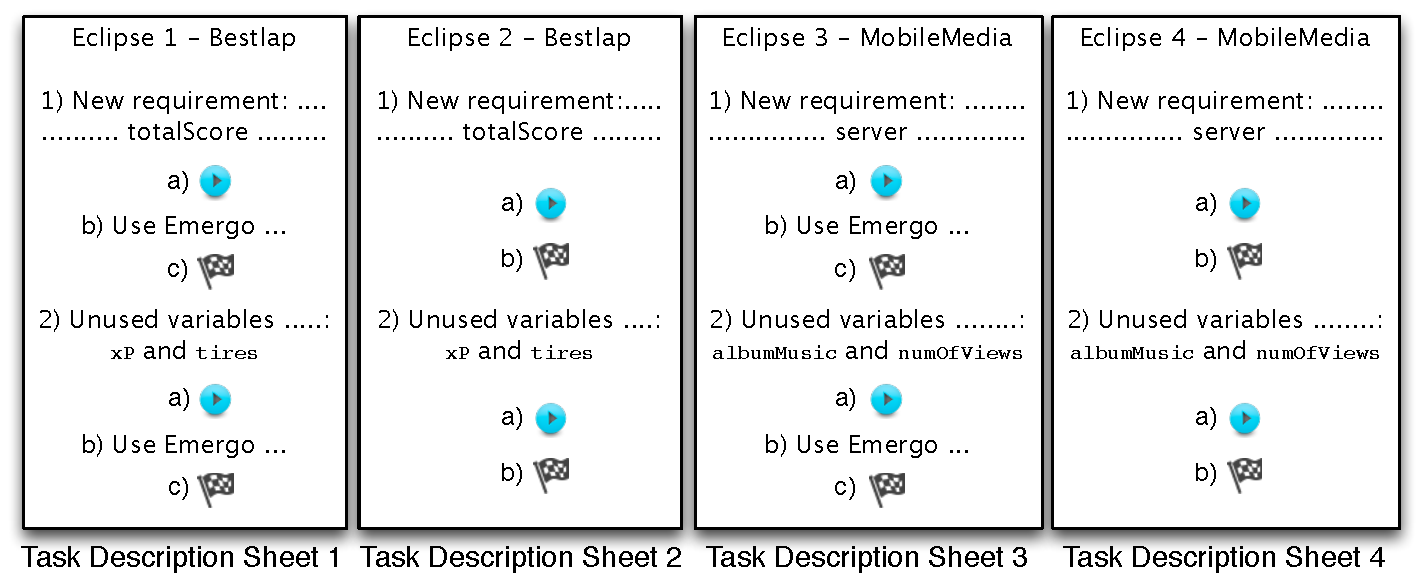
\includegraphics[width=\linewidth]{images/Maintenance-Tasks.pdf}
\caption{Task description sheets we distributed to the participants.}
\label{fig:maintenance-tasks}
\end{figure}

%\reviewer{As you point out the time penalty approach you use is rather arbitrary. While I can mostly accept your argument, I am less clear on why you chose to count number of errors for the unused variable task when participants were unable to test their results. This difference between using tests with the new requirements task and not having tests with the unused variables means the participants have a very different experience with each kind of task in using the emergent interfaces. I think the lack of tests for the unused variable tests moves far enough away from actual development that I do not think your results are very meaningful. The combination of the time penalty approach and the counting of errors without tests makes it unclear to me that the overall results of your experiments have sufficient validity.}

All times using emergent interfaces \textit{include} the time required by Emergo to compute these interfaces. Emergo takes, on the used systems, around $13$ seconds and $6$ seconds to generate emergent interfaces for Tasks 1 and~2, respectively. To compute interfaces for Tasks 3 and~4, we only need \textit{intraprocedural} analyses,  but, to simplify execution, instead of asking the developers to select the analysis to use, we let Emergo automatically apply \textit{interprocedural} ones. So, instead of 1 second or less (\textit{intraprocedural} analyses), it takes more time than needed, around 11, 16, 2, and 3 seconds for the variables \texttt{tires}, \texttt{xP}, \texttt{numberOfViews}, and \texttt{albumMusic}, respectively.

%However, notice that to compute emergent interfaces for the \textit{Unused variable} task, we do not need \textit{interprocedural} analyses. But to reduce complexity and thus avoid errors during the experiment, we do not ask developers to switch from \textit{interprocedural} to \textit{intraprocedural} analyses. So, Emergo generates all interfaces based on \textit{interprocedural} analyses, meaning that it spends more seconds than needed (when considering \textit{intraprocedural} analyses, Emergo takes around $1$ second or less).

To avoid the effect of software installed in different machines and related confounding parameters, we conduct the experiment in a virtual machine (executed on comparable hardware) that provides the same environment to all participants. All participants worked on the same time in the same room under the supervision of two experimenters.

%Each group uses a differently prepared version of Eclipse with or without emergent interfaces installed and with a prepared workspace for the Best Lap or MobileMedia task:
%\begin{itemize}
%
%	\item \textit{Eclipse 1:} Emergo installed; \textit{Best Lap} imported;
%	\item \textit{Eclipse 2:} Emergo not installed; \textit{Best Lap} imported;
%	\item \textit{Eclipse 3:} Emergo installed; \textit{MobileMedia} imported;
%	\item \textit{Eclipse 4:} Emergo not installed; \textit{MobileMedia} imported.
%
%\end{itemize}

%Providing these $4$ Eclipses aims to reduce problems during the experiment execution. For example, if we provide only one Eclipse with everything, the participant can use the wrong technique in the wrong SPL. Notice that each Eclipse represents one cell of our latin square design. We also have an additional Eclipse with Emergo installed and a toy SPL imported (\textit{JCalc}, a simple calculator) for the experiment dry-run.

%To understand the participants behavior, we recorded their screens in the \textit{Pilot} execution. We learned that they commit errors regarding tokens and statements such as ``//", ``\#", ``(" expression ``)", or \texttt{\#endif}, leading to many compilation errors. Since participants waste time dealing with these errors, they rather write the feature expressions in the task description sheets. Hence, the \textit{Unused variable} task does not have test cases. Again, in case Emergo is available, participants should use it. They also press \textit{Play} after reading the \textit{Unused variable} task.

%To form the latin squares, we randomly allocate participants to squares, then for each square we apply a different randomization to allocate treatments to each cell. After the randomization for all participants, we distribute the task sheets accordingly.

\subsection{Executions and Derivations}

At the start of the experiment session, we introduce preprocessors, the hiding facilities of virtual separation of concerns, and emergent interfaces. Together with the participants, we perform a warmup task that uses Emergo. We introduce how to use the \emph{Play/Pause} and \emph{Finish} buttons. For the entire experiment, we scheduled 2.5 hours (training, warmup, and execution). No deviations occurred.

%To make participants aware of preprocessors, VSoC, feature dependencies, emergent interfaces, and Emergo, we provide training before running the experiment, which takes around $1$ hour. Our idea consists of providing a minimum knowledge so that all participants can accomplish all tasks.
%We explain how to compute emergent interfaces using Emergo and how to navigate throughout the code using it. Then, we explain the buttons \textit{Play/Pause} and \textit{Finish}. We also discuss the target SPLs but we do not present any code of them. Finally, we inform they sometimes use Emergo and sometimes do not.

%After training, we distribute \textit{New requirement} and \textit{Unused variable} tasks based on the \textit{JCalc} toy SPL. Then, we execute a dry-run simulating the experiment, so participants use Emergo, projections that implement the VSoC idea, and the buttons exactly as if they are executing the experiment for real.


%!TEX root = ../main.tex

\section{Results and Discussion}

\label{sec:results}

Next we describe the results and test the hypotheses before discussing their implications (all raw results are available online, see Appendix~A). We proceed separately with the two tasks (new requirement and unused variable), reporting results from both rounds.

\subsection{New-requirement tasks}

We plot the times for both new-requirement tasks (1 and~2) with in Figure~\ref{fig:beanplots-nr}. Here we use beanplot batches, where each batch shows individual observations as small horizontal lines---the longest represents the average of that batch---and the density trace forms the batch shape. In Round~1 (see the legend in the figure), the slowest time when using emergent interfaces is still faster than the fastest time without. On average, participants accomplished the task \textit{3 times} faster with emergent interfaces. The key results were confirmed in the replication (emergent interfaces is, on average, 3.1 times faster), despite the different student levels. According to an ANOVA test, we obtain statistically significant evidence (see Appendix~B) that emergent interfaces reduce effort in both new-requirement tasks.

\begin{figure}[tp]
\centering
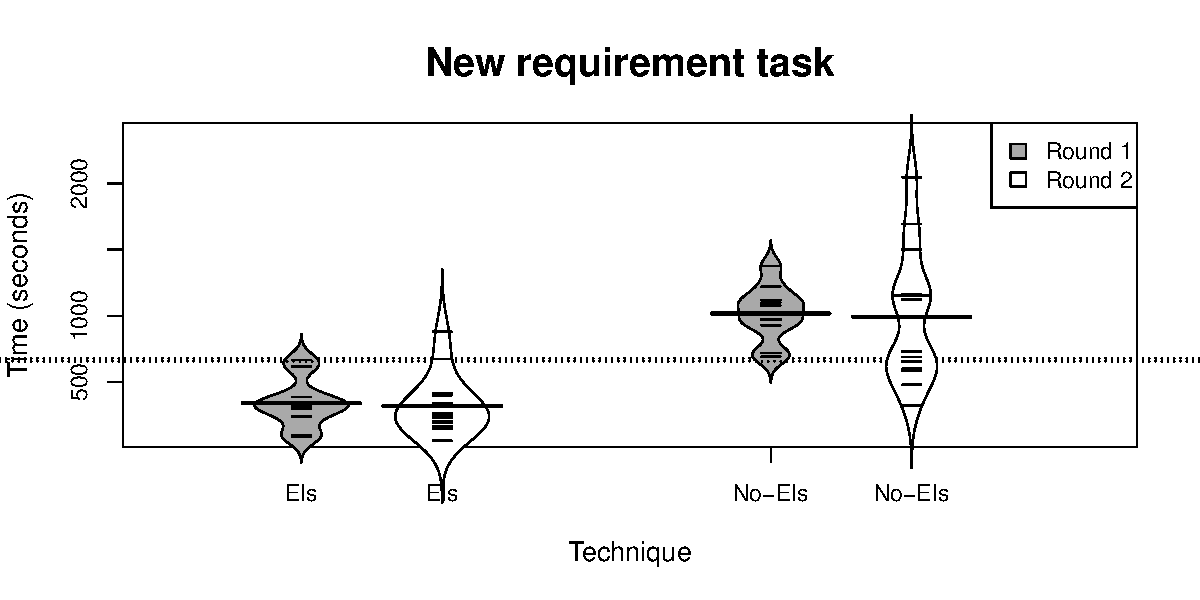
\includegraphics[width=0.5\textwidth]{images/Beanplots-NR.pdf}
\caption{Time results for the new-requirement task in both rounds.}
\label{fig:beanplots-nr}
\end{figure}

In Figure~\ref{fig:barplot-ne}, we plot the NE results for both new-requirement tasks. In Round~1, only one participant committed more errors when using emergent interfaces than without, and all of them committed errors when not using emergent interfaces (they thought they had finished the task but had not, potentially because they missed a dependency). The replication roughly confirms the results: $8$ ($57\%$) participants committed errors when not using emergent interfaces, but only $4$ ($28\%$) participants committed errors with emergent interfaces. Here we do not perform an ANOVA test on number of errors because we have many zero samples, being hard to observe a tendency and draw significant conclusions.

\begin{figure}[tp]
\centering
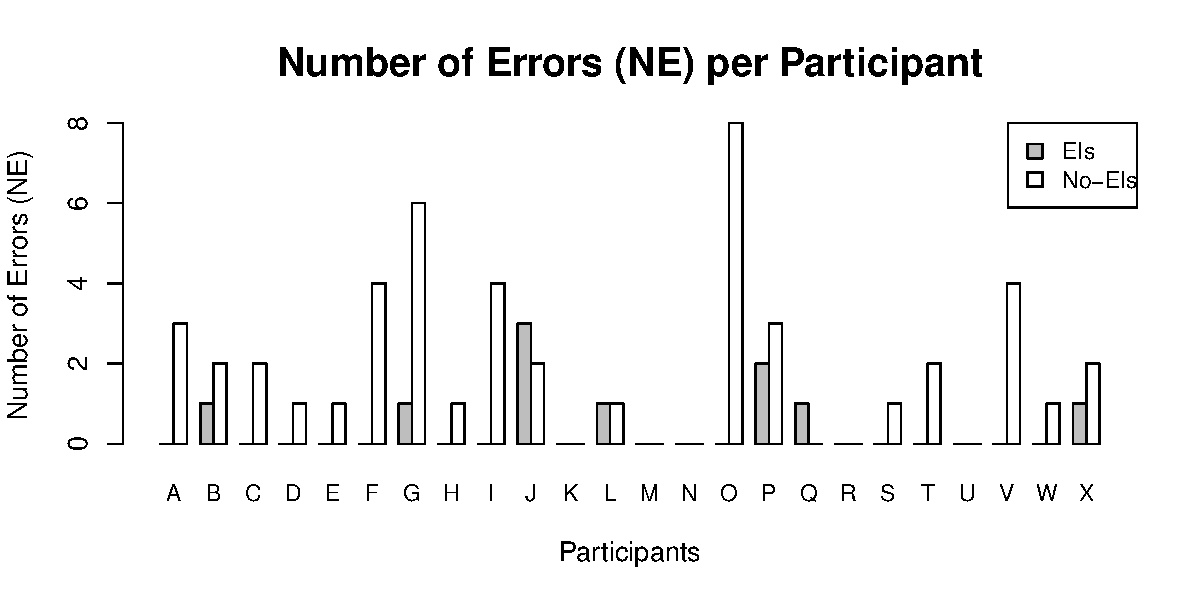
\includegraphics[width=0.5\textwidth]{images/Barplot-NE.pdf}
\caption{Number of Errors for the new-requirement task in both rounds. A-J: Round~1; K-X: Round~2.}
\label{fig:barplot-ne}
\end{figure}

\subsection{Unused-variable tasks}

Differently from the new-requirement task, here we do not have a test case, so we do not force participants to finish the task correctly. We make this important decision after reviewing the screen recordings from the pilot study. When fixing the unused variable problem, participants spend time since they miss statements such as \texttt{\#endif} and tokens like ``//" and ``\#", essential to compile the code and run the test, but typically less common when somebody is more familiar with the used notation. Because including this time would introduce bias into our results, we ask participants to write the \texttt{\#ifdef} feature expression in the task description sheets, not in the source code.
Thus, all participants finished the unused-variable task, but some committed errors when writing the feature expressions (so, NE $\neq 0$), which means we could have data of participants that, for example, did not try hard enough and consequently finished the task earlier. 

Regarding the measured time, it actually only reflects the time participants need until they think they are done.
To reflect incorrect solutions in the time, we could add a time penalty for incorrect tasks that simulates the extra time participants would have needed, if we mechanically reported the error or if they found the problem unfixed in practice.
As time penalty for an incorrect solution, we add the half the standard deviation of all participants times. We analyze both the original time (time until they think they are done) and the adjusted time with the penalty for incorrect tasks (which can be seen as a form of sensitivity analysis~\cite{statistics-sensitivity-analysis-book}).

%In summary, we are using a sensitivity analysis~\cite{sensitivity-analysis-issre02} to check what happens in our ANOVA tests if we change the time metric by adding the penalty.

%trying to estimate the real time to accomplish the task by

%help us on better understanding the influence of the penalty on the effort evaluation.

%we use a sensitivity analysis to assess the uncertainty in ou

%to be to able to run the ANOVA test. To do so, we use the standard deviation of all participants times in this task. \chk{REF}

%\chk{seems unsound to me. lets talk about this! if that's standard procedure explain so and give a reference! otherwise we mix our two dependent variables...}

%As the unused-variable task consists of fixing two unused variables, we consider it formed by two subtasks. The collected time data corresponds to a participant accomplishing both subtasks. So, we assume that participants spend the same time to accomplish both subtasks and add the time penalty as follows: if NE $= 2$, we add the standard deviation; if NE $= 1$, we add the standard deviation divided by two; if NE $= 0$, we add no penalty.

We plot the adjusted times for both unused-variable tasks (Tasks 3 and~4) in Figure~\ref{fig:beanplots-uv}. Differently from the new-requirement task, here the use of emergent interfaces adds little: the difference between the treatments is smaller. In fact, we obtain statistically significant evidence that emergent interfaces reduce effort only in the second round. The statistical results are stable for the original time (time until they think they are done) and the adjusted time. Regarding the adjusted time, the participants were {1.6 times} faster, on average.

%In Round~1, participants accomplished the task on average \textit{1.5 times} faster when using emergent interfaces. We confirmed the results in the replication, where participants were \textit{1.6 times} faster. Differently from the \textit{new-requirement} task, here the use of emergent interfaces adds little. We confirm this when running the ANOVA test: the difference between the treatments is not statistically significant on \textit{Round~1}. It is, however, in the replication (\textit{Round~2}).

When considering the product lines peculiarities, the \textit{MobileMedia} methods are simpler when compared to the \textit{Best Lap} ones. The time spent to accomplish the unused-variable task for the \textit{MobileMedia} variables is, on average, fairly similar when using and not using emergent interfaces. However, the difference is much greater for the \textit{Best Lap} variables: participants using emergent interfaces are \textit{2} and \textit{2.2 times} faster in the first and second rounds. Again, notice that the results are similar on both rounds.

%Notice that the difference between VSoC and emergent interfaces is not big when compared to the results of the \textit{new-requirement} maintenance task. On average, when using VSoC, participants are \textit{1.5 times} slower. Three participants ($30\%$) accomplished the maintenance task faster when using VSoC. When considering \textit{Round~2}, the difference is slightly higher: on average, when using VSoC, participants are \textit{1.68 times} slower. Four ($28\%$) participants that were faster when using VSoC.

\begin{figure}[tp]
\centering
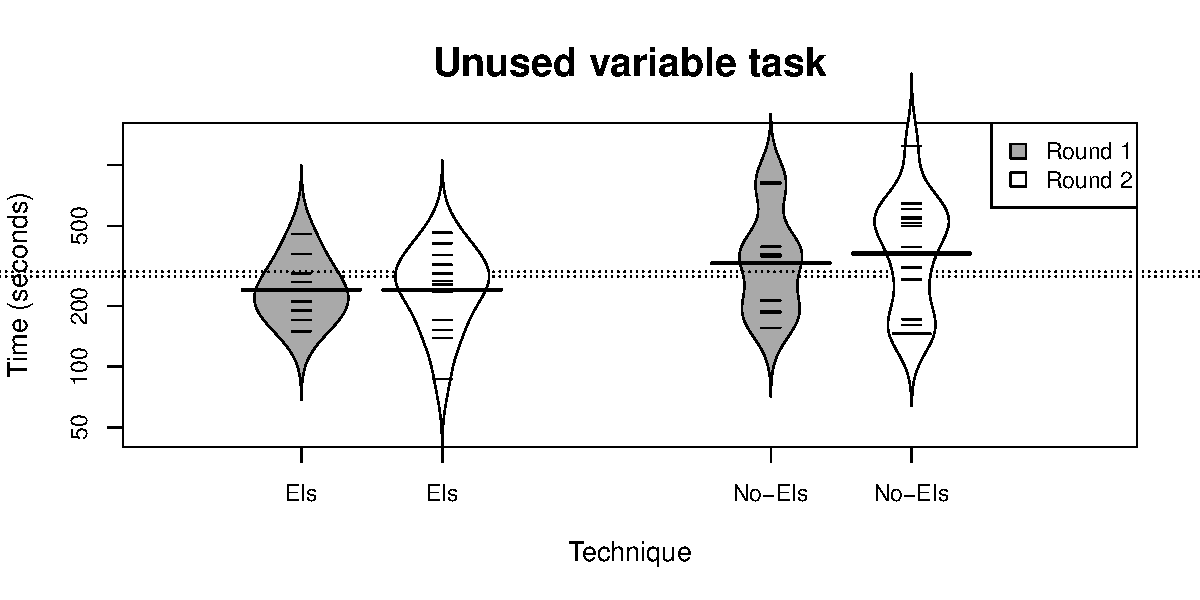
\includegraphics[width=0.5\textwidth]{images/Beanplots-UV.pdf}
\caption{Time results for the unused-variable task in both rounds.}
\label{fig:beanplots-uv}
\end{figure}

%Despite the differences (\textit{1.5} and \textit{1.68}), the ANOVA test points that the first one is not statistically significative (\textit{p-value} $= 0.13$), which leads us to not reject the null hypothesis for \textit{Round~1}. However, we do reject when considering \textit{Round~2}, since the \textit{p-value} for the technique factor is less than $0.05$. In particular, we have \textit{p-value} $= 0.016$.

%According to the Boxplot depicted in Figure~\ref{}, we have an outlier when using VSoC. To verify if this outlier changes our ANOVA test result, we replaced such a value by the VSoC time mean ($\mu = 443$ seconds) and did not add any penalty. Again, we reject the null hypothesis since \textit{p-value} $= 0.024$.

We plot the NE metric in Figure~\ref{fig:barplots-ne2}. The left-hand side represents Round~1; the right-hand side, Round~2. The errors consist of wrongly submitted \texttt{\#ifdef} statements. In general, it turns out that participants commit less errors when using emergent interfaces. The \textit{MobileMedia} methods are simpler, which might explain why participants commit less errors when performing the task in such product line.

\begin{figure}[tp]
\centering
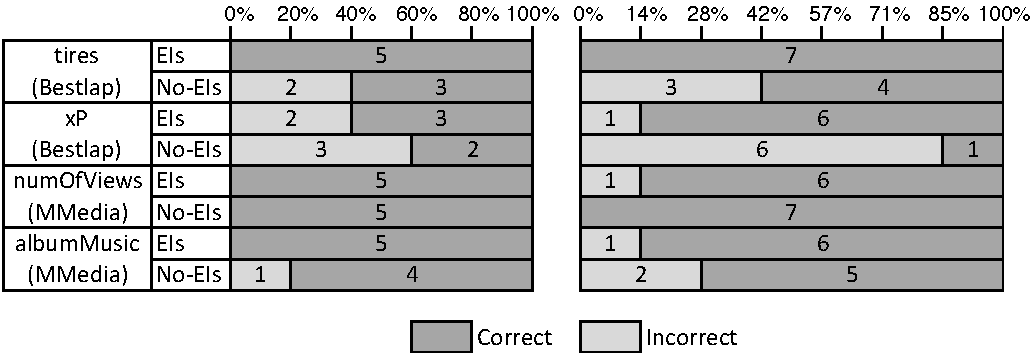
\includegraphics[width=0.5\textwidth]{images/Barplot-NE2.pdf}
\caption{Number of Errors for the unused-variable task in both rounds.}
\label{fig:barplots-ne2}
\end{figure}

%To identify other tendencies, we also performed a meta-analysis, jointly analyzing both rounds by combining their results. The differences are statistically significant for both tasks.

To identify other tendencies, we also performed a meta-analysis, where we combine and analyze both rounds results. The time differences are statistically significant for both tasks.

\subsection{Interpretation}

\paragraph{Effort reduction}
Regarding Question~1 (effort reduction), we found that emergent interfaces reduce the time spent to accomplish the new-requirement tasks. The difference is large with a three-fold improvement and statistically significant. Despite different student levels (graduate \textit{versus} undergraduate), the results are stable across both rounds.

We regard this as a confirmation that emergent interfaces make cross-feature dependencies explicit and help our participants to concentrate on the task, instead of navigating throughout the code to find and reason about dependencies. 

Additionally, we can see a qualitative difference between new-requirement tasks that require \textit{interprocedural} analysis across several methods and unused-variable tasks that require to analyze only code of a single method, where tasks involving \textit{interprocedural} analysis show higher speedups.
We argue that the effect is general to tasks with \textit{interprocedural} dependencies, since they are more difficult to follow without tool support. In contrast, emergent interfaces contribute comparably little over simple textual search tools when applied in the local context of a function, especially small ones. %In fact, we obtain statistically significant evidence in favor of emergent interfaces in only one round. 
Still, we can carefully interpret our results as suggesting that the effort gains might depend on the method complexity and size in the \textit{intraprocedural} context: speedups were considerably higher in the \textit{Best Lap} task, where variables were placed in longer methods. %When fixing the unused variables, developers spend fairly the same time (with and without emergent interfaces) on average for \textit{MobileMedia} variables. However, they are, on average, 2 times faster with emergent interfaces for the \textit{Best Lap} variables, which are placed at longer methods.


%However, they might get confused when Emergo shows many dependencies. Although we did not analyze this case, it turns out that this might not impact our conclusion. Indeed, developers spend more time to deal with dependencies in the Emergo views. On the other hand, developers also would spend more time to find many dependencies when using VSoC.
 %This situation gets worse if, from the maintenance point to the potentially impacted features, developers need to navigate through several method calls (the highest method call depth we have is $2$, see Table~\ref{tab:m1-characteristics}). 
%We have shown that emergent interfaces can play an important role on decreasing the \textit{effort} to locate these \textit{interprocedural} dependencies. 

In all cases, the performance gained from emergent interfaces outperforms the extra overhead required to compute them. Overall, we conclude that, for code change tasks involving cross-feature dependencies, emergent interfaces can help to reduce effort, while the actual effect size depends on the kind of task (\textit{interprocedural} or \textit{intraprocedural}, method size and complexity, etc).

%In summary, our results reveal a significative time difference in favor of emergent interfaces regarding the \textit{interprocedural} maintenance tasks we consider. But we should take the performance issue carefully into consideration, since it may change our results. In contrast, we can not observe many benefits when considering \textit{intraprocedural} tasks. However, depending on method characteristics like method size, number of features, and number of fragments, emergent interfaces can reduce \textit{Effort}. We also conclude that a method that contains alternative features can contribute to increase \textit{Effort} when using VSoC due to the time to reason about the feature model. emergent interfaces can also provide \textit{Effort} reduction when there is no dependency. The EI is empty. In contrast, developers using VSoC would unnecessarily search for dependencies that do not exist, increasing \textit{Effort}.


%However, there is a tradeoff. To achieve these benefits, Emergo needs to compute emergent interfaces in feasible time. Even though we did not notice any performance issue in our experiments, performance might be problem. To minimize this problem, we could apply optimizations into the Emergo algorithms. We could also pre-compute emergent interfaces and rely on caching algorithms.


%When considering the \textit{unused-variable} task, the time difference between VSoC and emergent interfaces is smaller when compared to the \textit{new-requirement} task. On average, VSoC is $1.5$ and $1.68$ times slower. Again, the results are pretty similar on both rounds. Nevertheless, we do not reject the null hypothesis on \textit{Round~1}. So, we can not expect many benefits when considering \textit{intraprocedural} dependencies. To find \textit{intraprocedural} dependencies in short methods, emergent interfaces adds little to standard tools like highlighting. However, we might observe \textit{Effort} reduction even in short methods. For example, when we have mutually exclusive features where the presence of \textit{A} prohibits the presence of \textit{B}. Since this information may not be explicit in source code, developers are susceptible to open, analyze, and even change features unnecessarily: if we maintain feature \textit{A}, there is no need to take \textit{B} as a potential impacted feature. Emergo executes feature-sensitive analyses, so dependencies between \textit{A} and \textit{B} are not taken into account. In contrast, VSoC users might spend time reasoning about the feature model.

\paragraph{Correctness}
Regarding Question~2 (reducing the number of errors made), our experiment suggests that emergent interfaces can reduce errors.

The \textit{new-requirement} task fits into an incomplete fix that has been pointed as a type of mistake in bug fixing~\cite{yin-fixes-become-bugs-fse11}. It is ``introduced by the fact that fixers may forget to fix all the buggy regions with the same root cause." Here the developer performs the code change in one feature but, due to cross-feature dependencies, she needs to change some other feature as well. If she does not change it, she introduces an error. To discover this kind of incomplete fix, developers should compile and execute one product with the problematic feature combination. Since there are so many potential product combinations, they might discover the error too late.

Given that emergent interfaces make developers aware of cross-feature dependencies, the chances of changing the impacted features increases, leading them to not press the \textit{Finish} button too rashly. This is consistent with recent research~\cite{yin-fixes-become-bugs-fse11}: ``If all such potential `influenced code' (either through control- or data-dependency) is clearly presented to developers, they may have better chances to detect the errors.'' Our results suggest that participants tend to introduce more errors without emergent interfaces. For unused-variable tasks, we can again observe that the longer methods of \textit{Best Lap} are more prone to errors than the shorter methods of \textit{MobileMedia}.

%Our results reveal that participants using VSoC also tend to wrongly write more feature expressions when compared to emergent interfaces: 75\% and 78\% (\textit{Round~1} and \textit{Round~2}). Because emergent interfaces point the features that use the variable we are fixing, it is easier to write the feature expression correctly. The majority of the errors happened for the \textit{Best Lap} variables, which are inside large methods: $87\%$ and $78\%$ of all wrongly written feature expressions occur for \textit{Best Lap} variables.

\paragraph{Outlook}
\label{sec:outlook}
First, Our experiment considered the influence of emergent interfaces in a specific scenario of preprocessor-based product lines. As we argued in Section~\ref{sec:motivating}, the concept can be generalized to enhance other implementation mechanisms with insufficient modularity mechanisms. Of course, we cannot simply transfer our results to these settings, but we are confident that, in follow-up experiments, we could find similar improvements also for task involving cross-feature dependencies in aspect- or feature-oriented implementations.

Second, our tasks were tailored to the specific capabilities of emergent interfaces. As discussed earlier, emergent interfaces address a narrow but important class of problems. We believe that it may actually be beneficial to run emergent interfaces in the background during any code changes and notify the user in any case the change would involve cross-feature dependencies. This way, a tool could lurk unnoticed in the background but would become active for specifically the kind of tasks we analyzed in our experiment to bring corresponding benefits regarding efficiency and correctness to those changes.

Finally, emergent interfaces have several capabilities that we did not explore in our experiment. For instance, in product lines often dependencies between features exist. Whereas a developer needs to manually search for dependencies and compare \texttt{\#ifdef} annotations on code statements with dependencies specified elsewhere, the underlying feature-sensitive data-flow analysis of Emergo can take such dependencies into account mechanically and automatically exclude infeasible paths (see Figure~\ref{fig:emergo-alternative}). Furthermore, even situations where Emergo derives empty interfaces can provide valuable information to users, indicating that they can stop their search; a fact that we did not evaluate yet.

\subsection{Threats to validity}

As in every experiment, there are several threats to validity. 
Most importantly, our experiment is limited to a specific implementation technique and specific code change scenarios, as discussed in Section~\ref{sec:outlook}; generalization to aspect-oriented languages and others requires further investigation; generalization to arbitrary maintenance tasks is not intended.

Second, our code change tasks are relatively simple (they take only few minutes to be accomplished). Nevertheless, we can still find bug reports regarding undeclared, uninitialized, and unused problems of single variables as well as of their uses along the code.\footnote{See \url{https://bugzilla.gnome.org/show_bug.cgi?id=580750}, \url{https://bugzilla.gnome.org/show_bug.cgi?id=445140}, \url{https://bugzilla.gnome.org/show_bug.cgi?id=309748}, \url{https://bugzilla.gnome.org/show_bug.cgi?id=461011}} Moreover, we claim that bigger tasks are formed by composing smaller ones. So, if we provide benefits for small tasks, it is plausible to consider that we can sum their times up and observe benefits for the whole task. Thus, we might carefully extrapolate our results to bigger tasks as well. Also, we analyze tasks on unfamiliar source code, whereas in practice developers might remember cross-feature dependencies from knowledge gained in prior tasks. 

% that is particularly sensitive to knowledge about feature dependencies. We argue that feature dependencies are important for many code change tasks in product lines, but cannot generalize to all code change tasks.

%Our results are specific to preprocessor-based implementations, and may potentially generalize to feature modules and aspects, though that requires further experiments.

Furthermore, recruiting students instead of professional developers as participants threats external validity. Though our students have some professional experience (60\,\% of our graduate students and 50\,\% of our undergraduate students reported industrial experience) and researchers have shown that graduate students can perform similar to professional developers~\cite{buse-students-experiments-sigplan-11}, we cannot generalize the results to other populations. The results are nevertheless relevant to emerging technology clusters, especially the ones in developing countries like Brazil, which are based on a young workforce with a significant percentage of part time students and recently graduated professionals.




%Our experiment focuses on simple tasks that only require changing variable values and conditional statements in the impacted fragments or fixing unused variable warnings. Despite having many other tasks we do not consider, our results may still hold for some other fine-grained tasks, like adding a new assignment to an existing variable and changing variable types.

Fourth, \textit{MobileMedia} is a small product line. We minimize this threat by also considering a real and commercial product line with \textit{Best Lap}. The results for both are consistent but we still need to consider more product lines. %However, it seems that characteristics like method size, complexity, and different kinds of feature dependencies predominate over the product line.

Emergent interfaces depend on data-flow analysis, which is potentially expensive to perform. In our experiments, we have included analysis time, but analysis time may not scale sufficiently with larger projects. In that case developers have to decide between imprecise results, precalculation in the background or in nightly builds, or advanced incremental computation strategies. When using imprecise analysis, the use of Emergo could even lead developers to a dangerous sense of security. In our experiment, analysis could be performed precisely in the reported moderate times.

Regarding construct validity, the time penalty that we add to wrong answers for the unused-variable task is potentially controversial. That way, the measured correctness influences the measured time. We argue that to provide the correct answer, participants would need more time and a test case, so the adjustment seems realistic. Also, we obtain similar statistical conclusions in both original and adjusted data.

%To avoid errors during the experiment, Emergo computes interfaces using exclusively \textit{interprocedural} analyses.  So, we are counting unnecessarily extra time for the \textit{unused-variable} task, which can also change the ANOVA test results.

Finally, regarding internal validity, we control many confounding parameters by keeping them constant (environment, tasks, domain knowledge) and by randomization. We reduce the influence of reading time by forcing participants to read the task before pressing the \textit{Play} button and the influence of writing time by making the actual changes small and simple. 

%The currently used data-flow analysis for product lines~\cite{} is not entirely precise. \chk{todo, discuss as threat to validity. emergo is imprecise? matter of performance?}
%Unfortunately, missing feature dependencies is not exclusively related to developers, but to our technique, due to the lack of completeness and precision of our data-flow analyses. Developers who rely on Emergo cannot perceive additional dependencies, which might lead them to introduce \textit{errors} to the product line. To minimize this limitation of our technique, we might consider many analyses to catch feature dependencies as much as possible. However, there is a tradeoff: better precision; lower performance.

%Since we used students, we should not generalize in principle our results to industry professionals. However, after the experiment, we asked whether they have already worked for a company or public institution as a programmer, and $6$ (60\%) MSc/PhD and $7$ (50\%) undergraduate students answered positively, varying from few months to many years of experience. Thus, we can carefully interpret our findings to experience developers as well. In fact, some studies have pointed out that using students as participants is a good surrogate for using industry professionals~\cite{buse-students-experiments-sigplan-11}.

%Our participants were not familiar with any source code. We believe that knowing it might change our results, since developers would be aware of dependencies regardless of using our technique. Nevertheless, we claim that, in a real product line like \textit{Best Lap}, it is unfeasible to know all dependencies, specially the fine-grained ones we consider. Thus, our results may still hold for developers familiar with the source code.

%The majority of the participants ($84\%$) did not know preprocessors either. But we can carefully generalize our results to developers familiar with this technique as well. Only the \textit{unused-variable} task requires participants manipulating \texttt{\#ifdef} expressions. The results point to high ratio of correctness, so our training and warmup seem enough. We believe that participants learn preprocessors quickly because it is a simple technique.

%We can carefully consider our results to methods that do not have feature dependencies, because developers using VSoC would search for dependencies that do not exist (consequently, not showed by the emergent interfaces), increasing \textit{effort}. However, the missing dependency threat also appears here: if Emergo misses dependencies, developers can introduce problems to the product line.

%!TEX root = ../main.tex

\section{Related work}

\label{sec:relatedwork}

%Emergent interfaces provide a tool-based alternative to language-based modularity mechanisms.


\paragraph{Preprocessor-based variability}
Preprocessor-based variability is common in industry (in fact likely the most common implementation form for product lines), even though its limitations regarding feature modularity are widely known and criticized~\cite{ifdef-harmful, F:EWSM95}. In this implementation form no interfaces exist between features.

Emergent interfaces follow a line of research works that try to provide tool-based solutions to help practitioners cope with existing preprocessor-infested code.
Virtual separation was explored with the tool CIDE, which can hide files and code fragments based on a given feature selection~\cite{christian-cide-icse08}. The version editor~\cite{ABGM:TSE02}, C-CLR~\cite{SGC:ACP4IS07}, and the Leviathan file system~\cite{HEBSL:FOSD11} show only projections of variable source code along similar lines. Similar ideas have also been explored outside the product-line context most prominently in Mylyn~\cite{murphy-mylyn-fse2006}, which learns from user behavior and creates tasked-based views (usually at the file level). Also in this context, emergent interfaces can help to make dependencies to hidden code fragments visible. 

Along those lines, several researchers investigated close-world whole-product-line analysis techniques that can type check or model all configurations of a product line in an efficient way~\cite{batory-safe-composition-gpce07,KATS:TOSEM11,KOE:OOPSLA12}. The underlying analysis of Emergo follows the general idea of whole-product-line analysis, but extends prior work this to data-flow analysis.

In our evaluation, we investigated only the influence of emergent interfaces, but not of other facets of preprocessor usage or virtual separation, which have been explored in prior complementary studies. Specifically, Feigenspan et al.\ have shown in a series of controlled experiments that different representations of conditional-compilation annotations can improve program comprehension~\cite{FKALSDPLS:ESE12}. Furthermore, Le et al.\ have shown in a controlled experiment that hiding irrelevant code fragments can improve understanding of product lines~\cite{erwig-harmful}---a result that analyzes with an ex-post analysis of using the version editor showing significant productivity increases~\cite{ABGM:TSE02}. These results complement each other and help building a tool environment for efficient maintenance of preprocessor-based implementations.

\paragraph{Feature modularity} Separating concerns in the implementation and hiding their internals has a long history in software-engineering research~\cite{parnas-criteria-cacm72} and programming language design~\cite{liskov-clu-77}. The research field has received significant attention with the focus on crosscutting concerns in the context of aspect-oriented programming~\cite{kiczales-aspectoriented-ecoop97}.

Early work on aspect-oriented programming was often criticized for neglecting modularity with clear interfaces~\cite{storzer-fragile-pointcut-04,S:OOPSLA06}, whereas more recently many researchers have investigated how to add additional interface mechanisms~\cite{aldrich-open-modules-ecoop05,SPAK:TOSEM10,GSSSTCR:IEEESoftware06,aspect-scope}, typically adding quite heavyweight language constructs. In contrast, our idea relies on tools to emerge interfaces on demand. So, developers do not need to write them in advance.

%\textbf{TODO: are there any languages where data-flow dependencies show up in interfaces, not only structural and type dependencies? is the next block something along those lines?}

Conceptual Modules~\cite{baniassad-conceptual-module-icse98} support analyzing the interface of a specific module---also using \textit{def-use} chains internally. Emergent interfaces extend conceptual modules by considering features relationships. Where conceptual modules were evaluated regarding correctness with case studies, we contribute a controlled experiment to evaluate correctness and reduced effort.



Emergent interfaces pursue an alternative, tool-based strategy, leaving the languages as is (at least until mainstream languages support modular crosscutting implementations), but providing tool support for developers. Eventually both directions may converge by using emergent interfaces to infer interfaces (similar to type inference, and with similar tradeoffs).



Overall, implicit and inferred interfaces, as computed by Emergo, might provide an interesting new point to explore feature modularity. Similar to the idea of virtual separation of concerns where we have no real separation but only emulate some form of modularity at tool level with views, emergent interfaces can emulate the benefits of real interfaces at a tool level. It cannot and does not want to replace a proper module system with explicit machine-checked interfaces~\cite{aldrich-open-modules-ecoop05,SPAK:TOSEM10,GSSSTCR:IEEESoftware06,CB:SPLC08}, but it can provide an interesting compromise between specification effort and usability~\cite{fosd11}.


\paragraph{Hidden dependencies}
Hidden dependencies are known to be problematic. This can be traced back to avoiding global variables~\cite{mary-shaw-global-variable-harmful-73}, where developers have no information over who uses their variables, since there is ``no mutual agreement between the creator and the accessor.'' In this context, developers are prone to introduce new errors during fixing activities~\cite{yin-fixes-become-bugs-fse11}, since information about the agreement is not available. Emergent interfaces support developers maintaining (variable) systems written in languages that do not provide strong interface mechanisms (between features). Indeed, the languages do not have such mechanisms for fine-grained crosscutting features such as the ones we often find in product lines.

\paragraph{Prior work on emergent interfaces}
We have first proposed emergent interfaces in an Onward! paper~\cite{ribeiro-emergent-onward10}. The prototype tool we introduced was based on CIDE~\cite{christian-cide-icse08} to annotate features and the reaching-definition analysis was approximated and unsound. It was neither \textit{interprocedural} nor even feature-sensitive, checking only whether the maintenance-point annotation was different of the reached statements' annotation. Subsequently, we assessed how often cross-feature dependencies occur in practice by mechanically mining 43 software systems with preprocessor variability~\cite{ribeiro-feature-dependencies-gpce11}, using an srcML-based infrastructure~\cite{liebig-40spls-icse10} conservatively approximating \textit{intraprocedural} data-flow using proxy metrics (unsound, but sufficient to approximate the frequency of the problem). Furthermore, we estimated potential effort reduction by a tool like Emergo, by  simulating code change tasks: we randomly selected variables from the $43$ systems and estimated developers effort by counting how many \texttt{\#ifdef} blocks they would analyze with and without emergent interfaces, showing a potential for significant reduction. 
In another branch of work, we investigated precise and efficient mechanisms for \emph{feature-sensitive} data-flow analyses~\cite{brabrand-dfa4spl-aosd12, brabrand-dfa4spl-taosd12, bodden-ifds4spl-pldi13}. These advances now form the technical infrastructure from which emergent interfaces are computed precisely (without unsound approximations of prior work).
In this paper, we bring together these results and focus on the originally envisioned application: emergent interfaces. We present a significantly revised and extended version of Emergo that uses \textit{intraprocedural} and \textit{interprocedural} analysis, and, for the first time, evaluate the actual benefit of emergent interfaces for code change tasks in a controlled experiment with human participants.

% Ignore tool papers!
%\idea{Christian, what about the emergo paper of the AOSD tool session? As far as I remember, I think that the main difference is that here we can execute emergo in real systems like best lap. In that paper, we used emergo in toys. Can we say that we 'significantly' extended Emergo? Not sure about that...}

%- emergo sem ser para software real

%In this paper, we revised and evolved the concept as well as the tool to implement it. In addition,  (last paragraph of the introduction)

%\textbf{TODO add a second or two expanding on the last paragraph on the introduction. be precise.}

%Emergo internally uses a variability-aware data-flow analysis that detects dependencies, even between code fragments that belong to different features. The product-line community has also investigated many analysis approaches for whole product lines, most prominently safe composition~\cite{batory-safe-composition-gpce07}, which performs type checking and detects corresponding dependencies. A product-line type system in CIDE can already raise type errors in specific configurations even if it relates to hidden code~\cite{KATS:TOSEM11}. Data-flow analysis in Emergo is more expensive to perform than type analysis, but gives also more precise interfaces.

\section{Concluding remarks}

In this paper we provide a full comprehension of emergent interfaces that emulate missing interfaces in many product line implementations. We provide a complete version of a tool capable of computing interfaces from data-flow analysis on demand. Emergent interfaces raise awareness of feature dependencies that are critical for maintaining (variable) software systems. With a conducted and replicated controlled experiment, we evaluate to what extent such tool support can help on achieving better feature modularization. Our study focuses on feature code change tasks in product lines implemented with preprocessors, since they are the prevalent way to implement variable software in industrial practice. We observe a significant decrease in code change effort by emergent interfaces, when faced with \textit{interprocedural} dependencies. Similarly, our study suggests a reduction in errors made during those code change tasks. In future work, we will focus on scaling the underlying data-flow analysis by trading off performance and precision, and investigate emergent interfaces for other implementation techniques.

%We introduce emergent interfaces that emulate missing interfaces in many product line implementations by computing interfaces from data-flow analysis on demand. 

%\reviewer{The conclusion says this paper introduces emergent interfaces. It really does not; previous papers did this.}

%\idea{Focus on the evaluation.}

%\section{Concluding remarks}
%
%In this paper we contributed to better understand to what extent tool-based support can help on achieving better feature modularization. We focused on preprocessors, since they are the prevalent way to implement variable software in industrial practice. Initially, we discussed problems related to feature dependencies. Then, we presented emergent interfaces and a tool support---named Emergo---to minimize these problems.
%
%To evaluate our proposal, we conducted and replicated an experiment that focuses on measuring development \textit{effort} and \textit{errors} introduction. The results are promising: we observed a large difference with a three-fold \textit{effort} reduction and statistically significant when using emergent interfaces for \textit{interprocedural} dependencies. When considering \textit{intraprocedural} dependencies, our results still reveal improvements (1.5 fold), but we confirmed statistical significance in only one replication. We also observed that, presenting feature dependencies is valuable, since it leads developers to avoid \textit{errors} introduction. In both rounds, our results and conclusions are similar despite the different students levels.
%
%Despite all the empirical evidence, we should be aware of the potential problems such as performance and missing dependencies. To avoid missing dependencies, developers can exchange performance for precision. They can configure Emergo to navigate deeper into method calls as well as take additional dataflow analyses into account. However, we might have both by reducing the depth and using Emergo iteratively by asking again for interfaces for each impacted feature.

%ACKNOWLEDGMENTS are optional
%\section{Acknowledgments}

%We would like to thank CNPq and National Institute of Science and Technology for Software Engineering (INES), for partially supporting this work. This work was also partially supported by ERC grant \#203099. Also, we thank SPG\footnote{\url{http://www.cin.ufpe.br/spg}} members for the fruitful discussions about this paper. We also thank Janet Siegmund for helpful comments on prior drafts of this paper.

%
% The following two commands are all you need in the
% initial runs of your .tex file to
% produce the bibliography for the citations in your paper.
\bibliographystyle{abbrv}
\bibliography{MMR}  % sigproc.bib is the name of the Bibliography in this case
% You must have a proper ".bib" file
%  and remember to run:
% latex bibtex latex latex
% to resolve all references
%
% ACM needs 'a single self-contained file'!
%
%APPENDICES are optional
%\balancecolumns

\appendix

\section{Additional materials}

All  data, materials, tasks, plug-ins, and R scripts can be found at \url{http://www.cin.ufpe.br/~mmr3/icse2014/}

\section{ANOVA tables}

In this appendix, we provide all ANOVA results.

\begin{table}[h]
\begin{center}
\footnotesize
\begin{tabular}{lrrrrr}
\hline
& Df & Sum Sq & Mean Sq & F value & $p\mbox{-}value$ \\
\hline
Replica & 4 & 276682 & 69171 & 2.3158 & 0.1451 \\
Replica:Subject & 5 & 193989 & 38798 & 1.2989 & 0.3528 \\
SPL & 1 & 5184 & 5184 & 0.1736 & 0.6879 \\
Technique & 1 & 2298420 & 2298420 & 76.9504 & {\bf 2.237e-05} \\
Residuals & 8 & 238951 & 29869 & & \\
\hline
\end{tabular}
\normalsize
\end{center}
\caption{Round 1 - New-requirement task.}
\label{tab:anova-r1-m1}
\end{table}

\begin{table}[h]
\begin{center}
\footnotesize
\begin{tabular}{lrrrrr}
\hline
& Df & Sum Sq & Mean Sq & F value & $p\mbox{-}value$ \\
\hline
Replica & 6 & 414.16 & 69.03 & 1.9960 & 0.1452 \\
Replica:Subject & 7 & 390.18 & 55.74 & 1.6118 & 0.2230 \\
Feature & 1 & 2.88 & 2.88 & 0.0833 & 0.7778 \\
Technique & 1 & 1286.46 & 1286.46 & 37.2003 & {\bf 5.343e-05} \\
Residuals & 12 & 414.99 & 34.58 & & \\
\hline
\end{tabular}
\normalsize
\end{center}
\caption{Round 2 - New-requirement task.}
\label{tab:anova-r2-m1}
\end{table}

\begin{table}[h]
\begin{center}
\footnotesize
\begin{tabular}{lrrrrr}
\hline
& Df & Sum Sq & Mean Sq & F value & $p\mbox{-}value$ \\
\hline
Replica & 4 & 57255 & 14314 & 0.4905 & 0.7435 \\
Replica:Subject & 5 & 260331 & 52066 & 1.7841 & 0.2223 \\
Feature & 1 & 61272 & 61272 & 2.0996 & 0.1854 \\
Technique & 1 & 82818 & 82818 & 2.8379 & {\bf 0.1306} \\
Residuals & 8 & 233465 & 29183 & & \\
\hline
\end{tabular}
\normalsize
\end{center}
\caption{Round 1 - Unused-variable task.}
\label{tab:anova-r1-m2}
\end{table}

\begin{table}[h]
\begin{center}
\footnotesize
\begin{tabular}{lrrrrr}
\hline
& Df & Sum Sq & Mean Sq & F value & $p\mbox{-}value$ \\
\hline
Replica & 6 & 81.516 & 13.586 & 0.8605 & 0.549665 \\
Replica:Subject & 7 & 267.751 & 38.250 & 2.4227 & 0.085284 \\
Feature & 1 & 173.000 & 173.000 & 10.9578 & 0.006221 \\
Technique & 1 & 123.068 & 123.068 & 7.7951 & {\bf 0.016285} \\
Residuals & 12 & 189.455 & 15.788 & & \\
\hline
\end{tabular}
\normalsize
\end{center}
\caption{Round 2 - Unused-variable task.}
\label{tab:anova-r2-m2}
\end{table}

\end{document}
